\documentclass[a4paper]{book}
\usepackage{makeidx}
\usepackage{graphicx}
\usepackage{multicol}
\usepackage{float}
\usepackage{listings}
\usepackage{color}
\usepackage{ifthen}
\usepackage[table]{xcolor}
\usepackage{textcomp}
\usepackage{alltt}
\usepackage{ifpdf}
\ifpdf
\usepackage[pdftex,
            pagebackref=true,
            colorlinks=true,
            linkcolor=blue,
            unicode
           ]{hyperref}
\else
\usepackage[ps2pdf,
            pagebackref=true,
            colorlinks=true,
            linkcolor=blue,
            unicode
           ]{hyperref}
\usepackage{pspicture}
\fi
\usepackage[utf8]{inputenc}
\usepackage[brazil]{babel}
\usepackage{mathptmx}
\usepackage[scaled=.90]{helvet}
\usepackage{courier}
\usepackage{sectsty}
\usepackage[titles]{tocloft}
\usepackage{doxygen}
\lstset{language=C++,inputencoding=utf8,basicstyle=\footnotesize,breaklines=true,breakatwhitespace=true,tabsize=4,numbers=left }
\makeindex
\setcounter{tocdepth}{3}
\renewcommand{\footrulewidth}{0.4pt}
\renewcommand{\familydefault}{\sfdefault}
\begin{document}
\hypersetup{pageanchor=false}
\begin{titlepage}
\vspace*{7cm}
\begin{center}
{\Large MC823 -\/ Laboratório de Redes: Trabalho 01 }\\
\vspace*{1cm}
{\large Gerado por Doxygen 1.7.4}\\
\vspace*{0.5cm}
{\small Quarta, 25 de Abril de 2012 23:42:04}\\
\end{center}
\end{titlepage}
\clearemptydoublepage
\pagenumbering{roman}
\tableofcontents
\clearemptydoublepage
\pagenumbering{arabic}
\hypersetup{pageanchor=true}
\chapter{Índice das Estruturas de Dados}
\section{Estruturas de Dados}
Aqui estão as estruturas de dados, uniões e suas respectivas descrições:\begin{DoxyCompactList}
\item\contentsline{section}{\hyperlink{structstr}{str} }{\pageref{structstr}}{}
\end{DoxyCompactList}

\chapter{Índice dos Arquivos}
\section{Lista de Arquivos}
Esta é a lista de todos os arquivos e suas respectivas descrições:\begin{DoxyCompactList}
\item\contentsline{section}{\hyperlink{beejClient_8c}{beejClient.c} }{\pageref{beejClient_8c}}{}
\item\contentsline{section}{\hyperlink{beejServer_8c}{beejServer.c} }{\pageref{beejServer_8c}}{}
\item\contentsline{section}{\hyperlink{mm_8c}{mm.c} }{\pageref{mm_8c}}{}
\item\contentsline{section}{\hyperlink{mm_8h}{mm.h} }{\pageref{mm_8h}}{}
\item\contentsline{section}{\hyperlink{resposta_8c}{resposta.c} }{\pageref{resposta_8c}}{}
\item\contentsline{section}{\hyperlink{resposta_8h}{resposta.h} }{\pageref{resposta_8h}}{}
\item\contentsline{section}{\hyperlink{str_8c}{str.c} }{\pageref{str_8c}}{}
\item\contentsline{section}{\hyperlink{str_8h}{str.h} }{\pageref{str_8h}}{}
\item\contentsline{section}{\hyperlink{tempo_8c}{tempo.c} }{\pageref{tempo_8c}}{}
\item\contentsline{section}{\hyperlink{tempo_8h}{tempo.h} }{\pageref{tempo_8h}}{}
\end{DoxyCompactList}

\chapter{Estruturas}
\hypertarget{structstr}{
\section{Referência da Estrutura str}
\label{structstr}\index{str@{str}}
}


{\ttfamily \#include $<$str.h$>$}

\subsection*{Campos de Dados}
\begin{DoxyCompactItemize}
\item 
char $\ast$ \hyperlink{structstr_a1fc4ce5d6a790001388349ca5b735383}{s}
\item 
size\_\-t \hyperlink{structstr_a047d84b55a2d3a9ef7fae84aec97fef2}{cur}
\item 
size\_\-t \hyperlink{structstr_ab653cd97c58cb798ab3e7e6c40e9f1df}{max}
\end{DoxyCompactItemize}


\subsection{Descrição Detalhada}
Estrutura de dados para armezar strings, e operações com strings. 

Definição na linha 19 do arquivo str.h.



\subsection{Campos}
\hypertarget{structstr_a047d84b55a2d3a9ef7fae84aec97fef2}{
\index{str@{str}!cur@{cur}}
\index{cur@{cur}!str@{str}}
\subsubsection[{cur}]{\setlength{\rightskip}{0pt plus 5cm}size\_\-t {\bf str::cur}}}
\label{structstr_a047d84b55a2d3a9ef7fae84aec97fef2}


Definição na linha 21 do arquivo str.h.

\hypertarget{structstr_ab653cd97c58cb798ab3e7e6c40e9f1df}{
\index{str@{str}!max@{max}}
\index{max@{max}!str@{str}}
\subsubsection[{max}]{\setlength{\rightskip}{0pt plus 5cm}size\_\-t {\bf str::max}}}
\label{structstr_ab653cd97c58cb798ab3e7e6c40e9f1df}


Definição na linha 22 do arquivo str.h.

\hypertarget{structstr_a1fc4ce5d6a790001388349ca5b735383}{
\index{str@{str}!s@{s}}
\index{s@{s}!str@{str}}
\subsubsection[{s}]{\setlength{\rightskip}{0pt plus 5cm}char$\ast$ {\bf str::s}}}
\label{structstr_a1fc4ce5d6a790001388349ca5b735383}


Definição na linha 20 do arquivo str.h.



A documentação para esta estrutura foi gerada a partir do seguinte arquivo:\begin{DoxyCompactItemize}
\item 
\hyperlink{str_8h}{str.h}\end{DoxyCompactItemize}

\chapter{Arquivos}
\hypertarget{beejClient_8c}{
\section{Referência do Arquivo beejClient.c}
\label{beejClient_8c}\index{beejClient.c@{beejClient.c}}
}
{\ttfamily \#include $<$stdio.h$>$}\par
{\ttfamily \#include $<$stdlib.h$>$}\par
{\ttfamily \#include $<$unistd.h$>$}\par
{\ttfamily \#include $<$errno.h$>$}\par
{\ttfamily \#include $<$string.h$>$}\par
{\ttfamily \#include $<$netdb.h$>$}\par
{\ttfamily \#include $<$sys/types.h$>$}\par
{\ttfamily \#include $<$netinet/in.h$>$}\par
{\ttfamily \#include $<$sys/socket.h$>$}\par
{\ttfamily \#include $<$arpa/inet.h$>$}\par
{\ttfamily \#include \char`\"{}tempo.h\char`\"{}}\par
{\ttfamily \#include \char`\"{}str.h\char`\"{}}\par
Gráfico de dependência de inclusões para beejClient.c:
\nopagebreak
\begin{figure}[H]
\begin{center}
\leavevmode
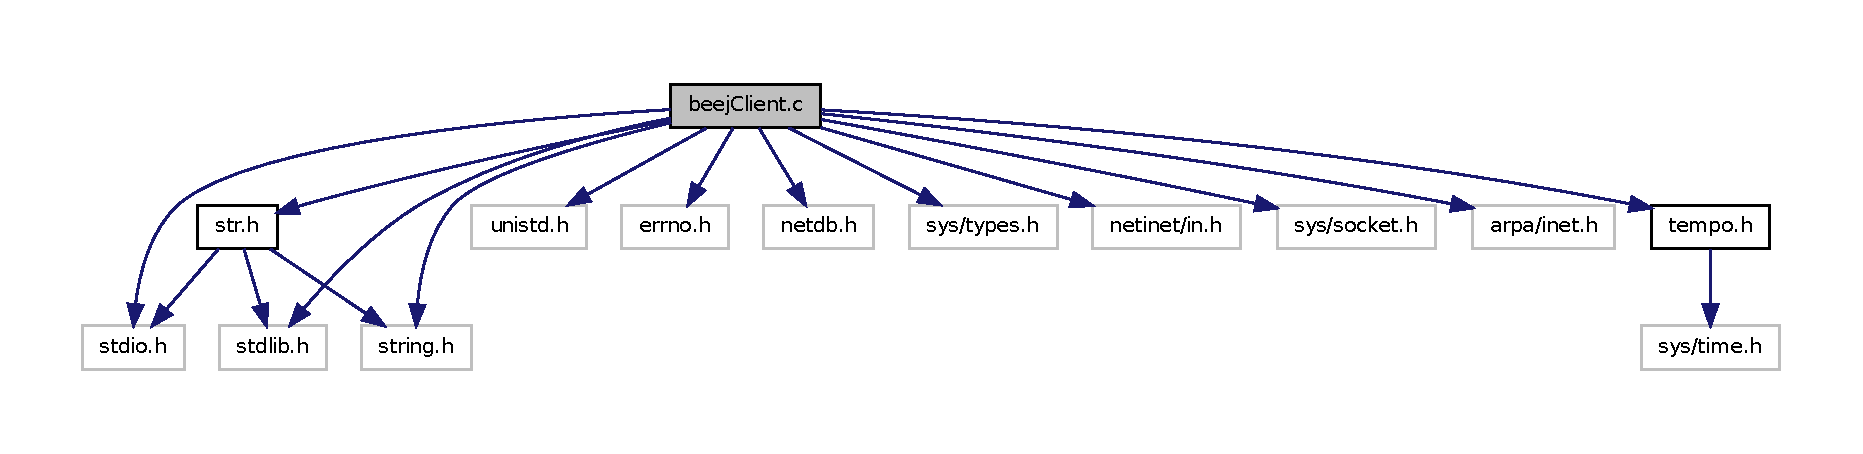
\includegraphics[width=400pt]{beejClient_8c__incl}
\end{center}
\end{figure}
\subsection*{Definições e Macros}
\begin{DoxyCompactItemize}
\item 
\#define \hyperlink{beejClient_8c_a614217d263be1fb1a5f76e2ff7be19a2}{PORT}~\char`\"{}39410\char`\"{}
\item 
\#define \hyperlink{beejClient_8c_a16c16f9369be4a374a3e621f6d13bb16}{MAXDATASIZE}~100
\end{DoxyCompactItemize}
\subsection*{Funções}
\begin{DoxyCompactItemize}
\item 
void \hyperlink{beejClient_8c_aead97c99e70c0da7036fbbe230ef68b6}{printUsage} ()
\item 
void $\ast$ \hyperlink{beejClient_8c_a294867ba9d7ff47e39d421134d8e12ab}{get\_\-in\_\-addr} (struct sockaddr $\ast$sa)
\item 
int \hyperlink{beejClient_8c_a0ddf1224851353fc92bfbff6f499fa97}{main} (int argc, char $\ast$argv\mbox{[}$\,$\mbox{]})
\end{DoxyCompactItemize}


\subsection{Definições e macros}
\hypertarget{beejClient_8c_a16c16f9369be4a374a3e621f6d13bb16}{
\index{beejClient.c@{beejClient.c}!MAXDATASIZE@{MAXDATASIZE}}
\index{MAXDATASIZE@{MAXDATASIZE}!beejClient.c@{beejClient.c}}
\subsubsection[{MAXDATASIZE}]{\setlength{\rightskip}{0pt plus 5cm}\#define MAXDATASIZE~100}}
\label{beejClient_8c_a16c16f9369be4a374a3e621f6d13bb16}


Definição na linha 22 do arquivo beejClient.c.

\hypertarget{beejClient_8c_a614217d263be1fb1a5f76e2ff7be19a2}{
\index{beejClient.c@{beejClient.c}!PORT@{PORT}}
\index{PORT@{PORT}!beejClient.c@{beejClient.c}}
\subsubsection[{PORT}]{\setlength{\rightskip}{0pt plus 5cm}\#define PORT~\char`\"{}39410\char`\"{}}}
\label{beejClient_8c_a614217d263be1fb1a5f76e2ff7be19a2}


Definição na linha 20 do arquivo beejClient.c.



\subsection{Funções}
\hypertarget{beejClient_8c_a294867ba9d7ff47e39d421134d8e12ab}{
\index{beejClient.c@{beejClient.c}!get\_\-in\_\-addr@{get\_\-in\_\-addr}}
\index{get\_\-in\_\-addr@{get\_\-in\_\-addr}!beejClient.c@{beejClient.c}}
\subsubsection[{get\_\-in\_\-addr}]{\setlength{\rightskip}{0pt plus 5cm}void$\ast$ get\_\-in\_\-addr (
\begin{DoxyParamCaption}
\item[{struct sockaddr $\ast$}]{sa}
\end{DoxyParamCaption}
)}}
\label{beejClient_8c_a294867ba9d7ff47e39d421134d8e12ab}
Função que obtem o endereço do socket

sa -\/ estrutura de dados do tipo sockaddr

endereço do socket (IPv4 ou IPv6) 

Definição na linha 60 do arquivo beejClient.c.



Este é o diagrama das funções que utilizam esta função:
\nopagebreak
\begin{figure}[H]
\begin{center}
\leavevmode
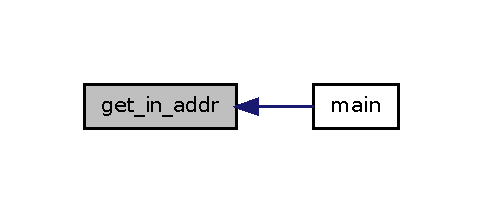
\includegraphics[width=232pt]{beejClient_8c_a294867ba9d7ff47e39d421134d8e12ab_icgraph}
\end{center}
\end{figure}


\hypertarget{beejClient_8c_a0ddf1224851353fc92bfbff6f499fa97}{
\index{beejClient.c@{beejClient.c}!main@{main}}
\index{main@{main}!beejClient.c@{beejClient.c}}
\subsubsection[{main}]{\setlength{\rightskip}{0pt plus 5cm}int main (
\begin{DoxyParamCaption}
\item[{int}]{argc, }
\item[{char $\ast$}]{argv\mbox{[}$\,$\mbox{]}}
\end{DoxyParamCaption}
)}}
\label{beejClient_8c_a0ddf1224851353fc92bfbff6f499fa97}
Função principal do cliente, que recebe parâmetros e os repassa ao servidor usando as funções send, e recupera a resposta do servidor usando a função send, imprimindo-\/a então na tela.

argc -\/ número de argumentos passados  argv\mbox{[}\mbox{]} -\/ argumentos passados

inteiro representando o sucesso da execução 

Definição na linha 82 do arquivo beejClient.c.



Este é o diagrama das funções utilizadas por esta função:
\nopagebreak
\begin{figure}[H]
\begin{center}
\leavevmode
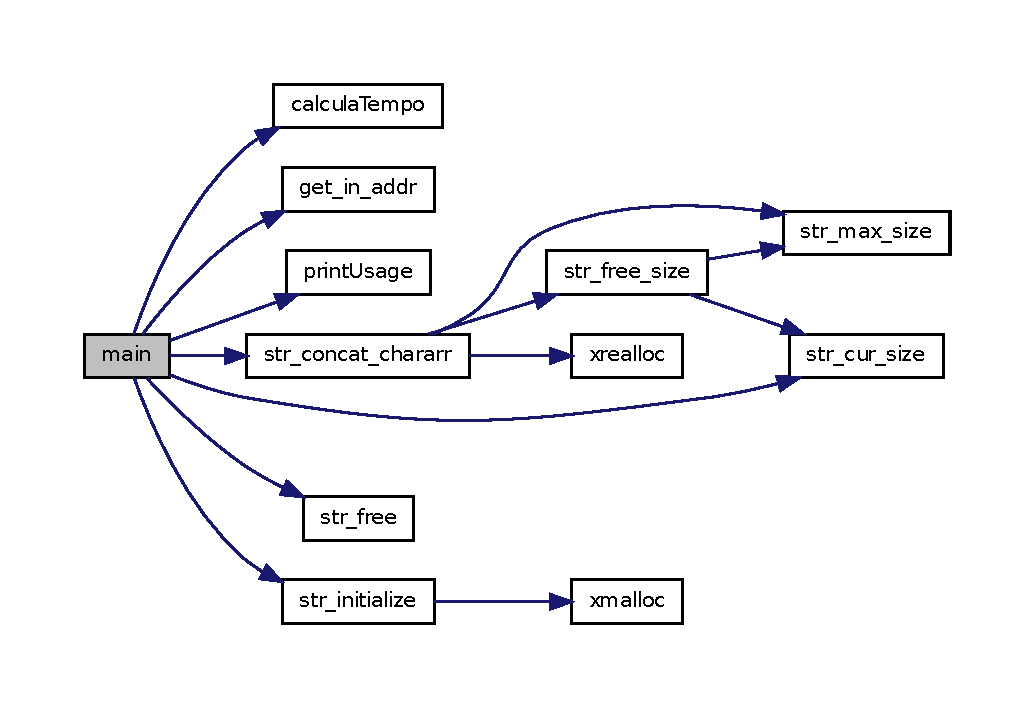
\includegraphics[width=400pt]{beejClient_8c_a0ddf1224851353fc92bfbff6f499fa97_cgraph}
\end{center}
\end{figure}


\hypertarget{beejClient_8c_aead97c99e70c0da7036fbbe230ef68b6}{
\index{beejClient.c@{beejClient.c}!printUsage@{printUsage}}
\index{printUsage@{printUsage}!beejClient.c@{beejClient.c}}
\subsubsection[{printUsage}]{\setlength{\rightskip}{0pt plus 5cm}void printUsage (
\begin{DoxyParamCaption}
{}
\end{DoxyParamCaption}
)}}
\label{beejClient_8c_aead97c99e70c0da7036fbbe230ef68b6}
Função auxiliar que imprime o modo de usar o programa 

Definição na linha 31 do arquivo beejClient.c.



Este é o diagrama das funções que utilizam esta função:
\nopagebreak
\begin{figure}[H]
\begin{center}
\leavevmode
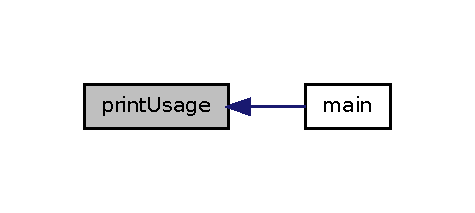
\includegraphics[width=228pt]{beejClient_8c_aead97c99e70c0da7036fbbe230ef68b6_icgraph}
\end{center}
\end{figure}



\hypertarget{beejServer_8c}{
\section{Referência do Arquivo beejServer.c}
\label{beejServer_8c}\index{beejServer.c@{beejServer.c}}
}
{\ttfamily \#include $<$stdio.h$>$}\par
{\ttfamily \#include $<$stdlib.h$>$}\par
{\ttfamily \#include $<$unistd.h$>$}\par
{\ttfamily \#include $<$errno.h$>$}\par
{\ttfamily \#include $<$string.h$>$}\par
{\ttfamily \#include $<$sys/types.h$>$}\par
{\ttfamily \#include $<$sys/socket.h$>$}\par
{\ttfamily \#include $<$netinet/in.h$>$}\par
{\ttfamily \#include $<$netdb.h$>$}\par
{\ttfamily \#include $<$arpa/inet.h$>$}\par
{\ttfamily \#include $<$sys/wait.h$>$}\par
{\ttfamily \#include $<$signal.h$>$}\par
{\ttfamily \#include \char`\"{}resposta.h\char`\"{}}\par
{\ttfamily \#include \char`\"{}tempo.h\char`\"{}}\par
Gráfico de dependência de inclusões para beejServer.c:
\nopagebreak
\begin{figure}[H]
\begin{center}
\leavevmode
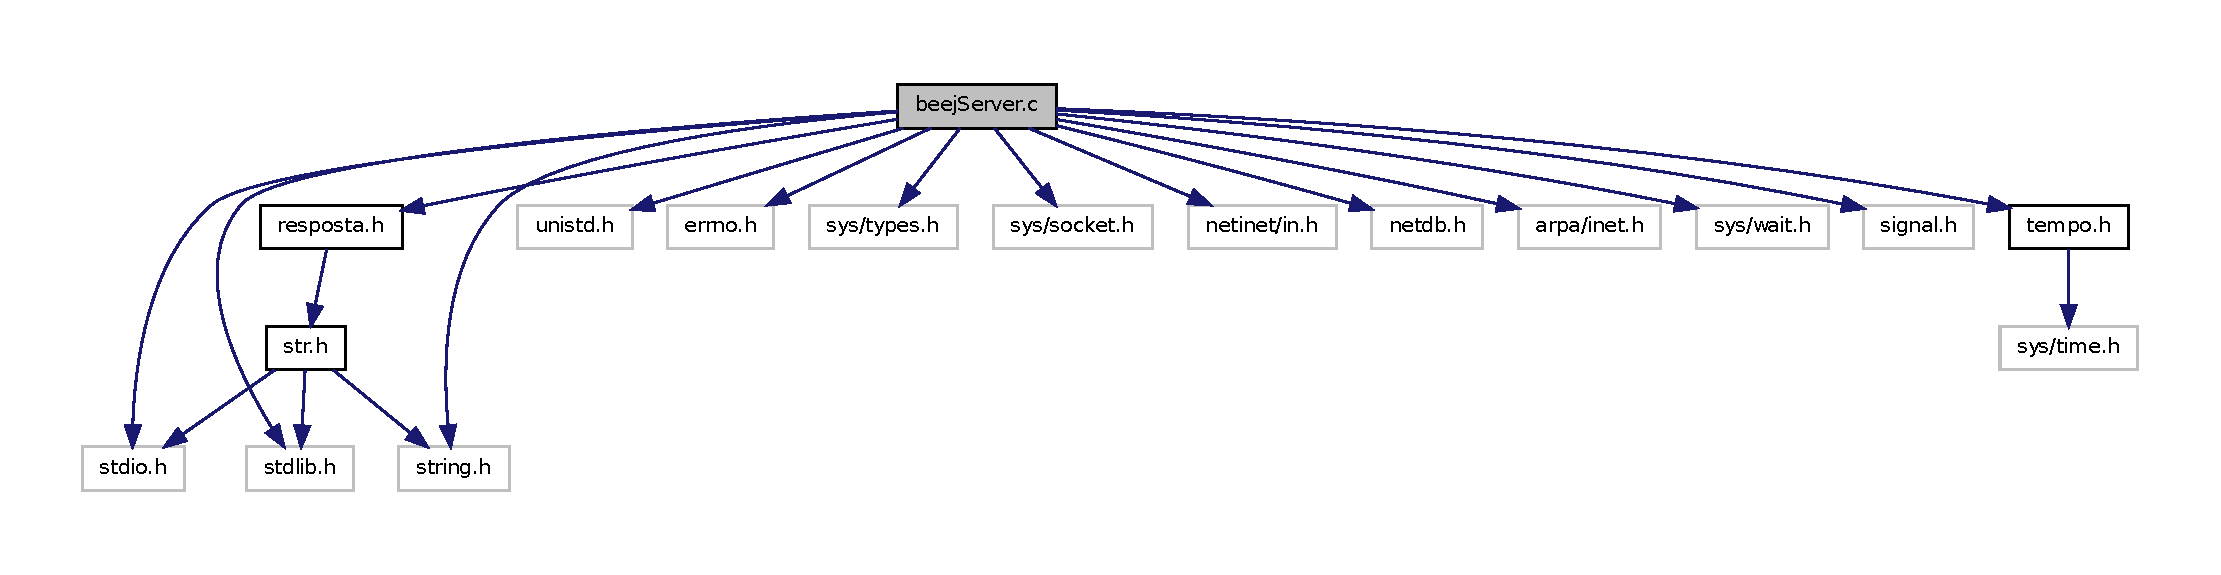
\includegraphics[width=400pt]{beejServer_8c__incl}
\end{center}
\end{figure}
\subsection*{Definições e Macros}
\begin{DoxyCompactItemize}
\item 
\#define \hyperlink{beejServer_8c_a614217d263be1fb1a5f76e2ff7be19a2}{PORT}~\char`\"{}39410\char`\"{}
\item 
\#define \hyperlink{beejServer_8c_aeefbbafa97642defe3ee6c3080b7d66f}{BACKLOG}~10
\item 
\#define \hyperlink{beejServer_8c_a16c16f9369be4a374a3e621f6d13bb16}{MAXDATASIZE}~100
\end{DoxyCompactItemize}
\subsection*{Funções}
\begin{DoxyCompactItemize}
\item 
void \hyperlink{beejServer_8c_a6c2d9589ac70568b8e3a6980bb3d45d6}{sigchld\_\-handler} (int s)
\item 
void $\ast$ \hyperlink{beejServer_8c_a294867ba9d7ff47e39d421134d8e12ab}{get\_\-in\_\-addr} (struct sockaddr $\ast$sa)
\item 
int \hyperlink{beejServer_8c_a840291bc02cba5474a4cb46a9b9566fe}{main} (void)
\end{DoxyCompactItemize}


\subsection{Definições e macros}
\hypertarget{beejServer_8c_aeefbbafa97642defe3ee6c3080b7d66f}{
\index{beejServer.c@{beejServer.c}!BACKLOG@{BACKLOG}}
\index{BACKLOG@{BACKLOG}!beejServer.c@{beejServer.c}}
\subsubsection[{BACKLOG}]{\setlength{\rightskip}{0pt plus 5cm}\#define BACKLOG~10}}
\label{beejServer_8c_aeefbbafa97642defe3ee6c3080b7d66f}


Definição na linha 22 do arquivo beejServer.c.

\hypertarget{beejServer_8c_a16c16f9369be4a374a3e621f6d13bb16}{
\index{beejServer.c@{beejServer.c}!MAXDATASIZE@{MAXDATASIZE}}
\index{MAXDATASIZE@{MAXDATASIZE}!beejServer.c@{beejServer.c}}
\subsubsection[{MAXDATASIZE}]{\setlength{\rightskip}{0pt plus 5cm}\#define MAXDATASIZE~100}}
\label{beejServer_8c_a16c16f9369be4a374a3e621f6d13bb16}


Definição na linha 23 do arquivo beejServer.c.

\hypertarget{beejServer_8c_a614217d263be1fb1a5f76e2ff7be19a2}{
\index{beejServer.c@{beejServer.c}!PORT@{PORT}}
\index{PORT@{PORT}!beejServer.c@{beejServer.c}}
\subsubsection[{PORT}]{\setlength{\rightskip}{0pt plus 5cm}\#define PORT~\char`\"{}39410\char`\"{}}}
\label{beejServer_8c_a614217d263be1fb1a5f76e2ff7be19a2}


Definição na linha 21 do arquivo beejServer.c.



\subsection{Funções}
\hypertarget{beejServer_8c_a294867ba9d7ff47e39d421134d8e12ab}{
\index{beejServer.c@{beejServer.c}!get\_\-in\_\-addr@{get\_\-in\_\-addr}}
\index{get\_\-in\_\-addr@{get\_\-in\_\-addr}!beejServer.c@{beejServer.c}}
\subsubsection[{get\_\-in\_\-addr}]{\setlength{\rightskip}{0pt plus 5cm}void$\ast$ get\_\-in\_\-addr (
\begin{DoxyParamCaption}
\item[{struct sockaddr $\ast$}]{sa}
\end{DoxyParamCaption}
)}}
\label{beejServer_8c_a294867ba9d7ff47e39d421134d8e12ab}
Função que obtem o endereço do socket

sa -\/ estrutura de dados do tipo sockaddr

endereço do socket (IPv4 ou IPv6) 

Definição na linha 52 do arquivo beejServer.c.

\hypertarget{beejServer_8c_a840291bc02cba5474a4cb46a9b9566fe}{
\index{beejServer.c@{beejServer.c}!main@{main}}
\index{main@{main}!beejServer.c@{beejServer.c}}
\subsubsection[{main}]{\setlength{\rightskip}{0pt plus 5cm}int main (
\begin{DoxyParamCaption}
\item[{void}]{}
\end{DoxyParamCaption}
)}}
\label{beejServer_8c_a840291bc02cba5474a4cb46a9b9566fe}
Função que controla o fluxo de execução do servidor, recebendo os parâmetros passados pelo cliente, montando uma resposta de acordo com esses parâmetros, e devolvendo essa resposta ao cliente

inteiro indicando se o fluxo de execução do programa foi bem sucedido 

Definição na linha 72 do arquivo beejServer.c.



Este é o diagrama das funções utilizadas por esta função:
\nopagebreak
\begin{figure}[H]
\begin{center}
\leavevmode
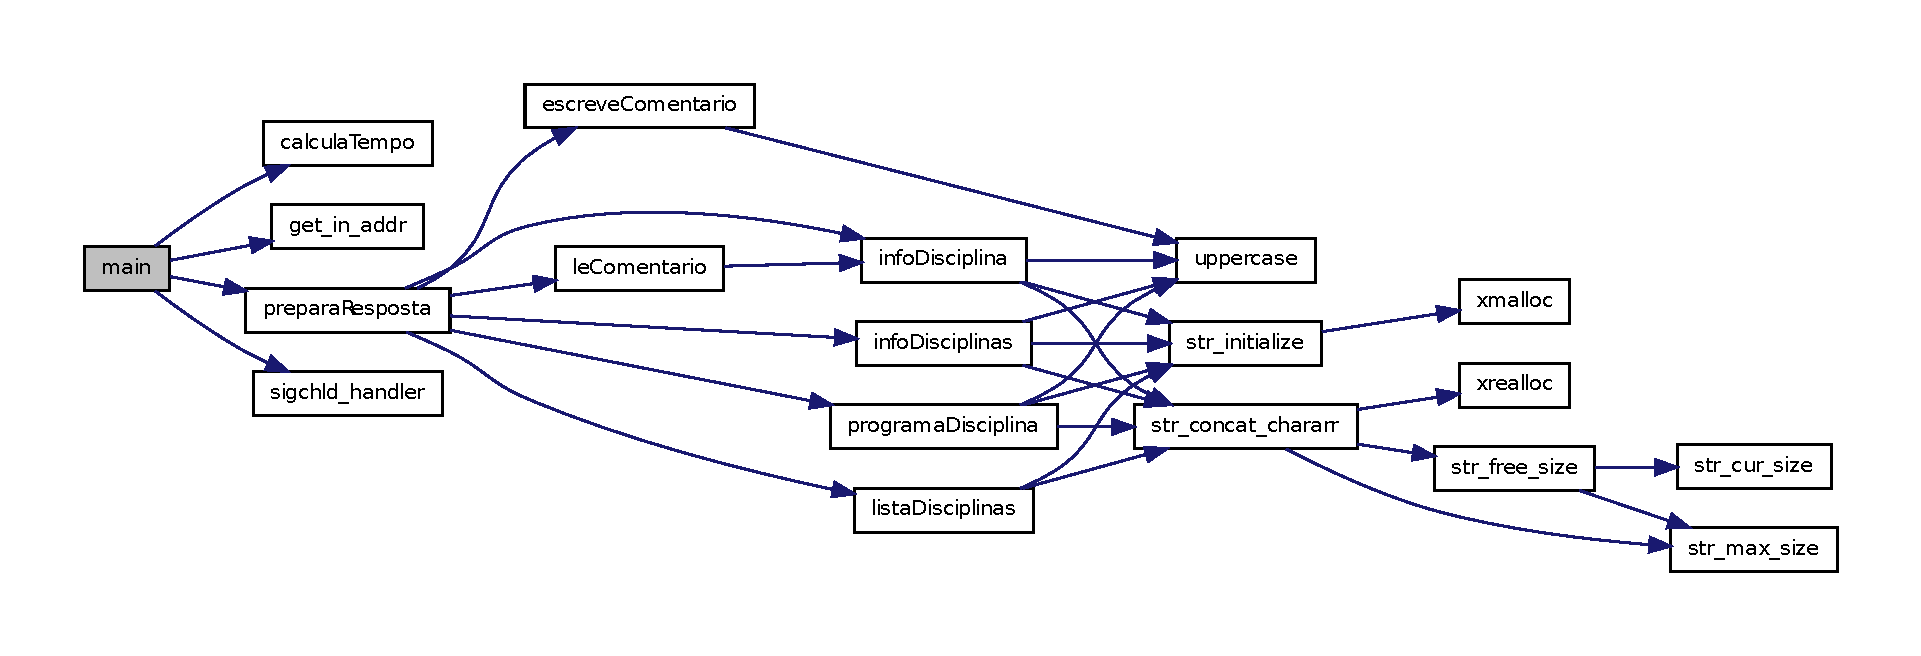
\includegraphics[width=400pt]{beejServer_8c_a840291bc02cba5474a4cb46a9b9566fe_cgraph}
\end{center}
\end{figure}


\hypertarget{beejServer_8c_a6c2d9589ac70568b8e3a6980bb3d45d6}{
\index{beejServer.c@{beejServer.c}!sigchld\_\-handler@{sigchld\_\-handler}}
\index{sigchld\_\-handler@{sigchld\_\-handler}!beejServer.c@{beejServer.c}}
\subsubsection[{sigchld\_\-handler}]{\setlength{\rightskip}{0pt plus 5cm}void sigchld\_\-handler (
\begin{DoxyParamCaption}
\item[{int}]{s}
\end{DoxyParamCaption}
)}}
\label{beejServer_8c_a6c2d9589ac70568b8e3a6980bb3d45d6}
Função auxiliar para controlar os processos filhos

s -\/ flag 

Definição na linha 36 do arquivo beejServer.c.



Este é o diagrama das funções que utilizam esta função:
\nopagebreak
\begin{figure}[H]
\begin{center}
\leavevmode
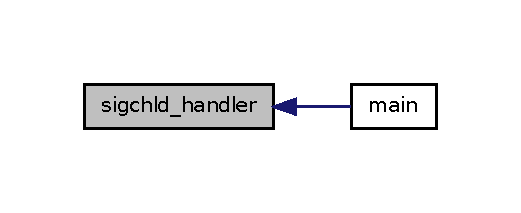
\includegraphics[width=250pt]{beejServer_8c_a6c2d9589ac70568b8e3a6980bb3d45d6_icgraph}
\end{center}
\end{figure}



\hypertarget{mm_8c}{
\section{Referência do Arquivo mm.c}
\label{mm_8c}\index{mm.c@{mm.c}}
}
{\ttfamily \#include $<$stdio.h$>$}\par
{\ttfamily \#include $<$stdlib.h$>$}\par
Gráfico de dependência de inclusões para mm.c:
\nopagebreak
\begin{figure}[H]
\begin{center}
\leavevmode
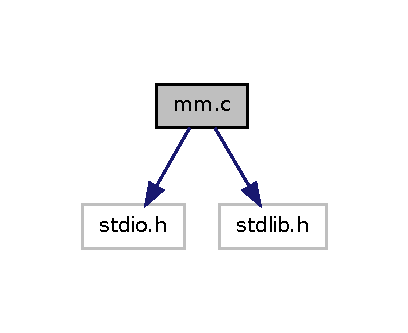
\includegraphics[width=196pt]{mm_8c__incl}
\end{center}
\end{figure}
\subsection*{Funções}
\begin{DoxyCompactItemize}
\item 
void $\ast$ \hyperlink{mm_8c_a42ccfa6fc49cc4ce90cc44cd05052490}{xmalloc} (size\_\-t size)
\item 
void $\ast$ \hyperlink{mm_8c_a93a8ec6e8a6eef0f62b7e5b50d0bf9e4}{xrealloc} (void $\ast$ptr, size\_\-t size)
\end{DoxyCompactItemize}


\subsection{Funções}
\hypertarget{mm_8c_a42ccfa6fc49cc4ce90cc44cd05052490}{
\index{mm.c@{mm.c}!xmalloc@{xmalloc}}
\index{xmalloc@{xmalloc}!mm.c@{mm.c}}
\subsubsection[{xmalloc}]{\setlength{\rightskip}{0pt plus 5cm}void$\ast$ xmalloc (
\begin{DoxyParamCaption}
\item[{size\_\-t}]{size}
\end{DoxyParamCaption}
)}}
\label{mm_8c_a42ccfa6fc49cc4ce90cc44cd05052490}
Função auxiliar que aloca memória.

size -\/ tamanho a ser alocado

inteiro representando sucesso ou fracasso 

Definição na linha 14 do arquivo mm.c.



Este é o diagrama das funções que utilizam esta função:
\nopagebreak
\begin{figure}[H]
\begin{center}
\leavevmode
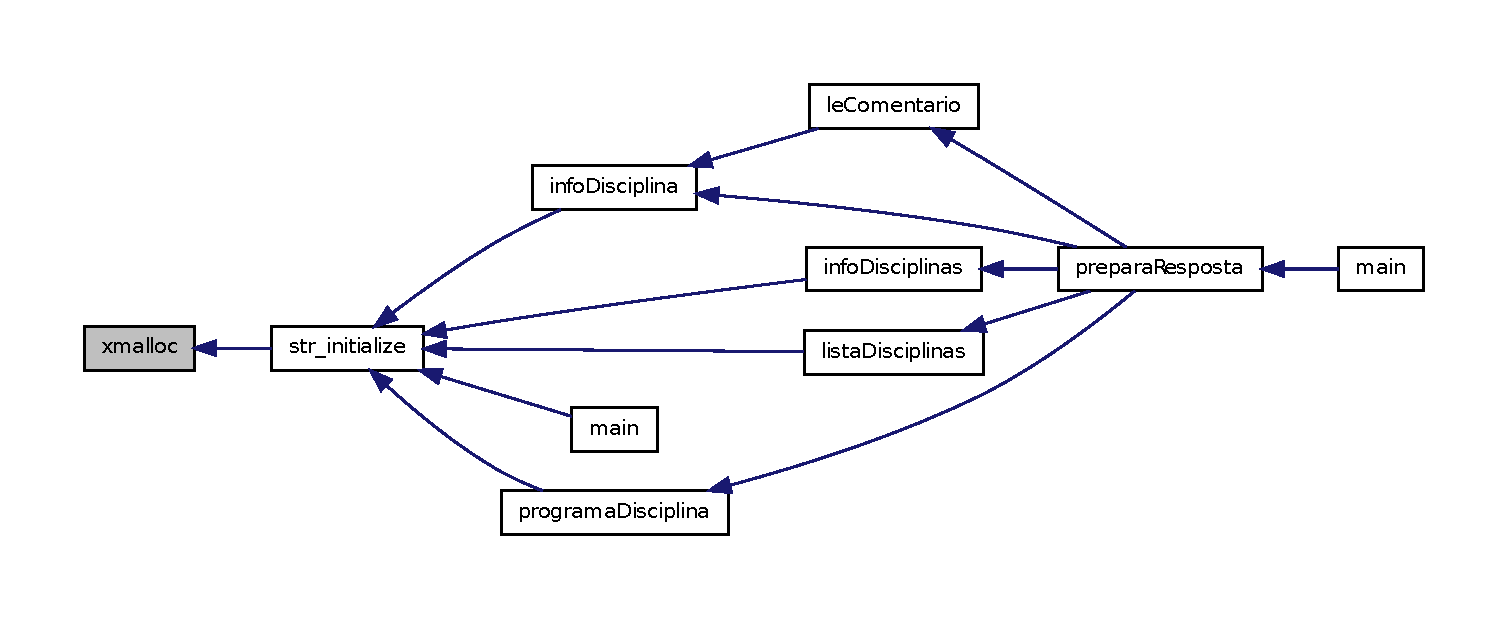
\includegraphics[width=400pt]{mm_8c_a42ccfa6fc49cc4ce90cc44cd05052490_icgraph}
\end{center}
\end{figure}


\hypertarget{mm_8c_a93a8ec6e8a6eef0f62b7e5b50d0bf9e4}{
\index{mm.c@{mm.c}!xrealloc@{xrealloc}}
\index{xrealloc@{xrealloc}!mm.c@{mm.c}}
\subsubsection[{xrealloc}]{\setlength{\rightskip}{0pt plus 5cm}void$\ast$ xrealloc (
\begin{DoxyParamCaption}
\item[{void $\ast$}]{ptr, }
\item[{size\_\-t}]{size}
\end{DoxyParamCaption}
)}}
\label{mm_8c_a93a8ec6e8a6eef0f62b7e5b50d0bf9e4}
Função auxiliar usada para realocar memória

ptr -\/ ponteiro para a estrutura a ser realocada  size -\/ tamanho a ser realocado

inteiro representando sucesso ou fracasso 

Definição na linha 34 do arquivo mm.c.



Este é o diagrama das funções que utilizam esta função:
\nopagebreak
\begin{figure}[H]
\begin{center}
\leavevmode
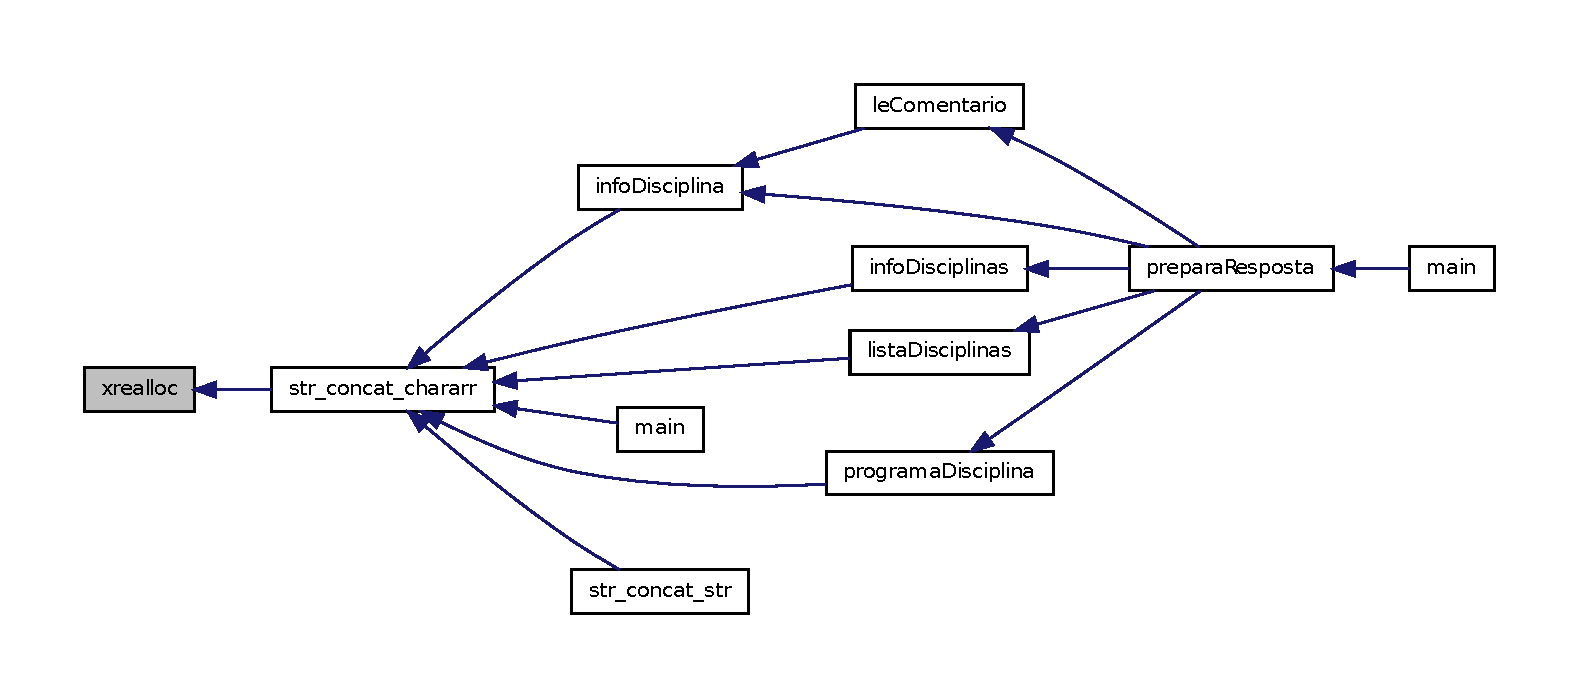
\includegraphics[width=400pt]{mm_8c_a93a8ec6e8a6eef0f62b7e5b50d0bf9e4_icgraph}
\end{center}
\end{figure}



\hypertarget{mm_8h}{
\section{Referência do Arquivo mm.h}
\label{mm_8h}\index{mm.h@{mm.h}}
}
{\ttfamily \#include $<$stdlib.h$>$}\par
Gráfico de dependência de inclusões para mm.h:
\nopagebreak
\begin{figure}[H]
\begin{center}
\leavevmode
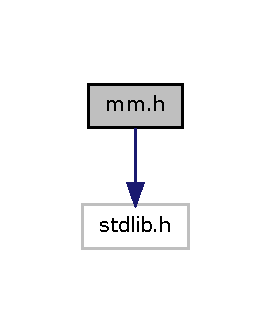
\includegraphics[width=130pt]{mm_8h__incl}
\end{center}
\end{figure}
Este grafo mostra quais arquivos estão direta ou indiretamente relacionados com este arquivo:
\nopagebreak
\begin{figure}[H]
\begin{center}
\leavevmode
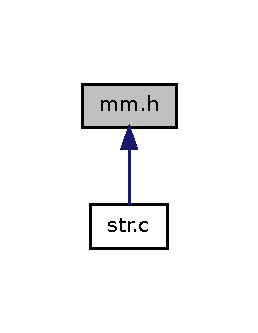
\includegraphics[width=124pt]{mm_8h__dep__incl}
\end{center}
\end{figure}
\subsection*{Funções}
\begin{DoxyCompactItemize}
\item 
void $\ast$ \hyperlink{mm_8h_a42ccfa6fc49cc4ce90cc44cd05052490}{xmalloc} (size\_\-t size)
\item 
void $\ast$ \hyperlink{mm_8h_a613e35ff7dff52c1870a25e888777c19}{xrealloc} (void $\ast$ptr, size\_\-t newsize)
\end{DoxyCompactItemize}


\subsection{Funções}
\hypertarget{mm_8h_a42ccfa6fc49cc4ce90cc44cd05052490}{
\index{mm.h@{mm.h}!xmalloc@{xmalloc}}
\index{xmalloc@{xmalloc}!mm.h@{mm.h}}
\subsubsection[{xmalloc}]{\setlength{\rightskip}{0pt plus 5cm}void$\ast$ xmalloc (
\begin{DoxyParamCaption}
\item[{size\_\-t}]{size}
\end{DoxyParamCaption}
)}}
\label{mm_8h_a42ccfa6fc49cc4ce90cc44cd05052490}
Função auxiliar que aloca memória.

size -\/ tamanho a ser alocado

inteiro representando sucesso ou fracasso 

Definição na linha 14 do arquivo mm.c.



Este é o diagrama das funções que utilizam esta função:
\nopagebreak
\begin{figure}[H]
\begin{center}
\leavevmode
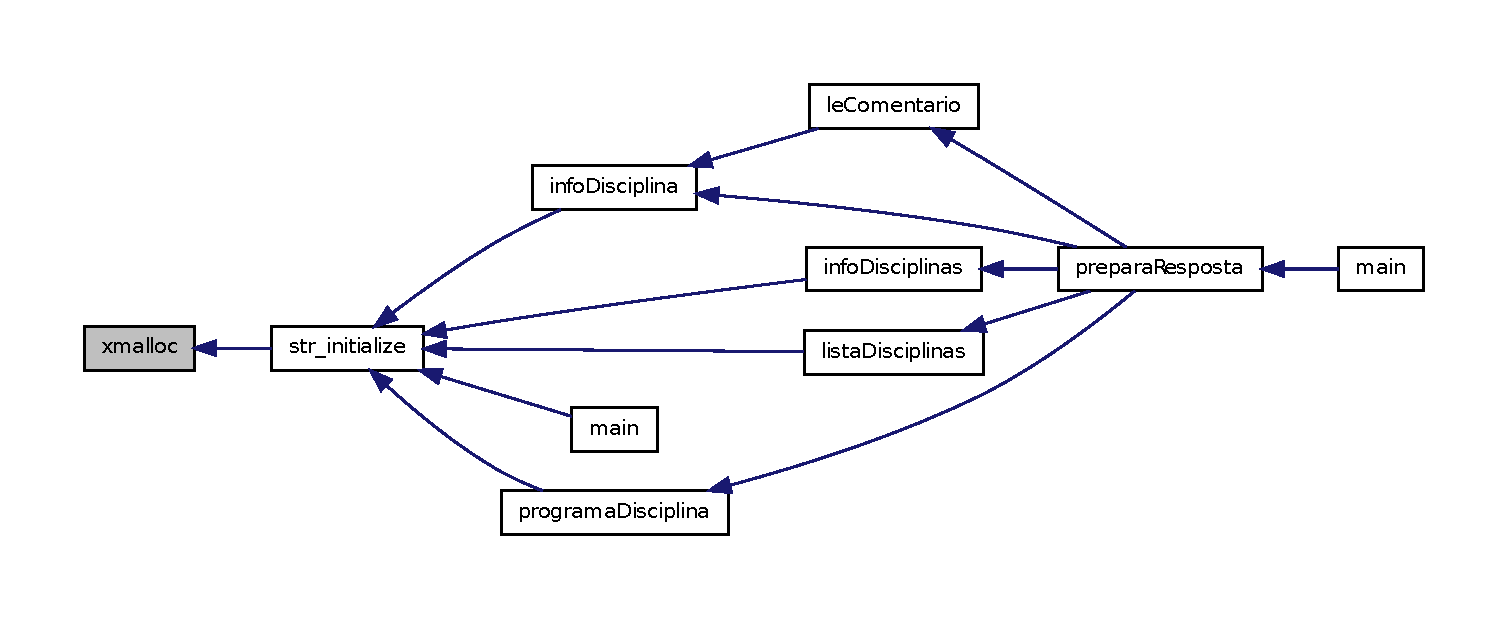
\includegraphics[width=400pt]{mm_8h_a42ccfa6fc49cc4ce90cc44cd05052490_icgraph}
\end{center}
\end{figure}


\hypertarget{mm_8h_a613e35ff7dff52c1870a25e888777c19}{
\index{mm.h@{mm.h}!xrealloc@{xrealloc}}
\index{xrealloc@{xrealloc}!mm.h@{mm.h}}
\subsubsection[{xrealloc}]{\setlength{\rightskip}{0pt plus 5cm}void$\ast$ xrealloc (
\begin{DoxyParamCaption}
\item[{void $\ast$}]{ptr, }
\item[{size\_\-t}]{size}
\end{DoxyParamCaption}
)}}
\label{mm_8h_a613e35ff7dff52c1870a25e888777c19}
Função auxiliar usada para realocar memória

ptr -\/ ponteiro para a estrutura a ser realocada  size -\/ tamanho a ser realocado

inteiro representando sucesso ou fracasso 

Definição na linha 34 do arquivo mm.c.



Este é o diagrama das funções que utilizam esta função:
\nopagebreak
\begin{figure}[H]
\begin{center}
\leavevmode
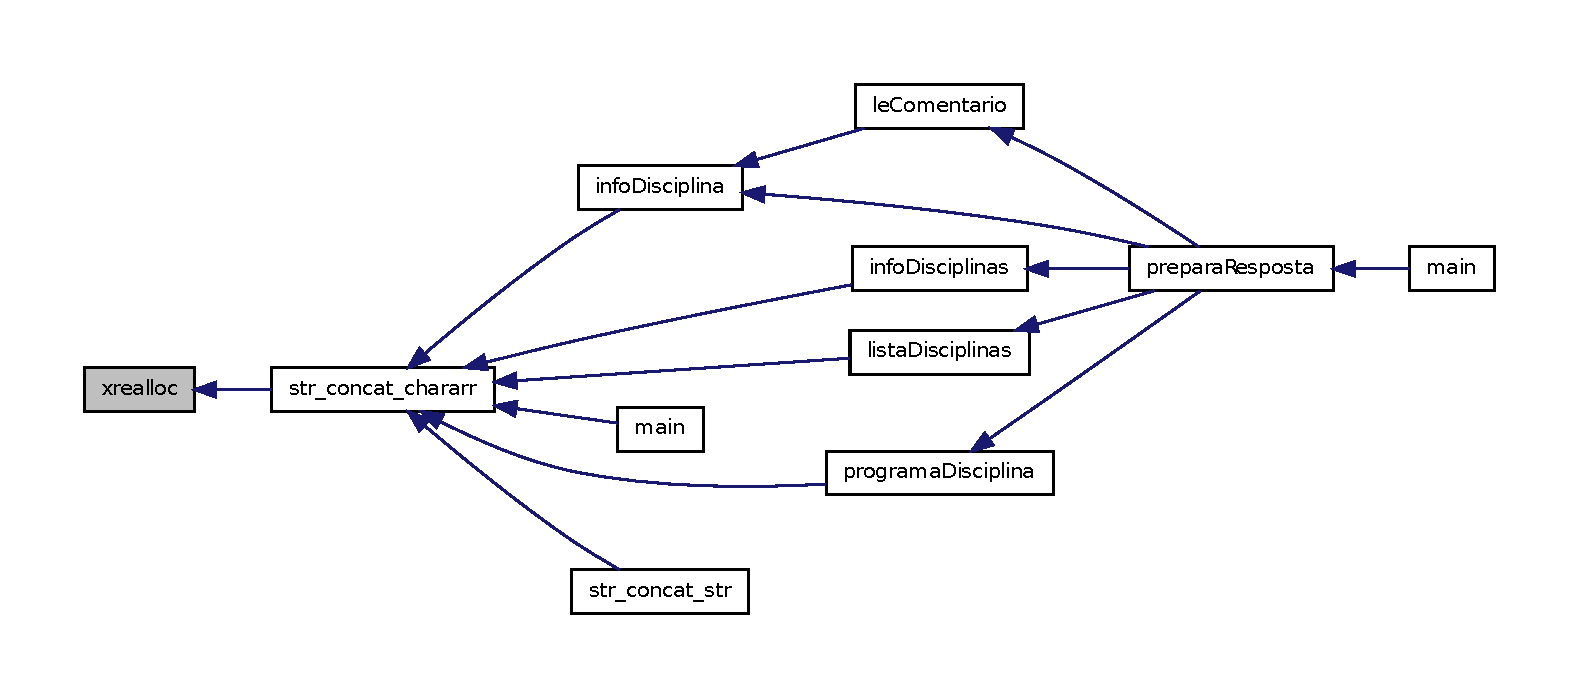
\includegraphics[width=400pt]{mm_8h_a613e35ff7dff52c1870a25e888777c19_icgraph}
\end{center}
\end{figure}



\hypertarget{resposta_8c}{
\section{Referência do Arquivo resposta.c}
\label{resposta_8c}\index{resposta.c@{resposta.c}}
}
{\ttfamily \#include \char`\"{}resposta.h\char`\"{}}\par
{\ttfamily \#include $<$string.h$>$}\par
Gráfico de dependência de inclusões para resposta.c:
\nopagebreak
\begin{figure}[H]
\begin{center}
\leavevmode
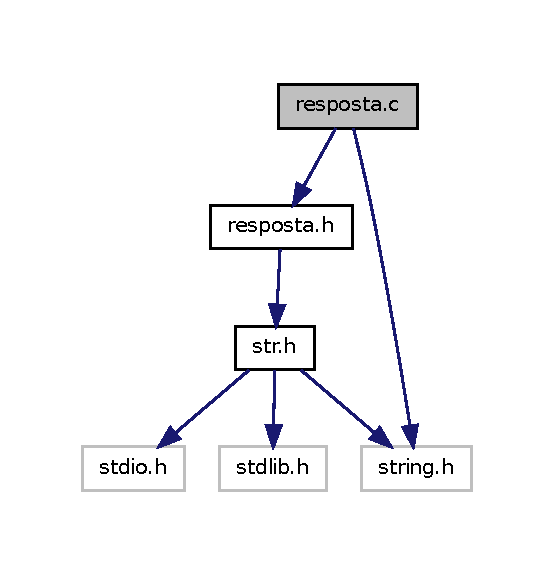
\includegraphics[width=266pt]{resposta_8c__incl}
\end{center}
\end{figure}
\subsection*{Definições e Macros}
\begin{DoxyCompactItemize}
\item 
\#define \hyperlink{resposta_8c_a281d136eba7bc38021f2fccbf61a633f}{NUM\_\-MAX\_\-DISCIPLINAS}~10
\item 
\#define \hyperlink{resposta_8c_a5d429b813e4525632cd4064f5e47213e}{TAM\_\-MAX\_\-NOME\_\-DISCIPLINA}~120
\end{DoxyCompactItemize}
\subsection*{Funções}
\begin{DoxyCompactItemize}
\item 
char $\ast$ \hyperlink{resposta_8c_a9bb7e31e6340d62b3afb839655847563}{preparaResposta} (char $\ast$buf)
\item 
char $\ast$ \hyperlink{resposta_8c_a2a098bc71f2a19dd74318fd778676979}{leComentario} (char $\ast$disc)
\item 
char $\ast$ \hyperlink{resposta_8c_a2b6f397b0bfae5590b292d282513c54b}{escreveComentario} (char $\ast$disc, char $\ast$comentario)
\item 
char $\ast$ \hyperlink{resposta_8c_adca402fde30bac4845d32a7dd4e6160a}{listaDisciplinas} ()
\item 
char $\ast$ \hyperlink{resposta_8c_ae53e5d927eddd073efa7dd3777c222c2}{programaDisciplina} (char $\ast$disc)
\item 
char $\ast$ \hyperlink{resposta_8c_aae0e9c217f1ede36bbf9821b36bba3f9}{infoDisciplinas} ()
\item 
char $\ast$ \hyperlink{resposta_8c_a6c04d45a3b24b43c86d50889bde25d67}{infoDisciplina} (char $\ast$disc)
\item 
void \hyperlink{resposta_8c_aaf2c986b7320373a463f607a67c07365}{uppercase} (char $\ast$sPtr)
\end{DoxyCompactItemize}


\subsection{Definições e macros}
\hypertarget{resposta_8c_a281d136eba7bc38021f2fccbf61a633f}{
\index{resposta.c@{resposta.c}!NUM\_\-MAX\_\-DISCIPLINAS@{NUM\_\-MAX\_\-DISCIPLINAS}}
\index{NUM\_\-MAX\_\-DISCIPLINAS@{NUM\_\-MAX\_\-DISCIPLINAS}!resposta.c@{resposta.c}}
\subsubsection[{NUM\_\-MAX\_\-DISCIPLINAS}]{\setlength{\rightskip}{0pt plus 5cm}\#define NUM\_\-MAX\_\-DISCIPLINAS~10}}
\label{resposta_8c_a281d136eba7bc38021f2fccbf61a633f}


Definição na linha 4 do arquivo resposta.c.

\hypertarget{resposta_8c_a5d429b813e4525632cd4064f5e47213e}{
\index{resposta.c@{resposta.c}!TAM\_\-MAX\_\-NOME\_\-DISCIPLINA@{TAM\_\-MAX\_\-NOME\_\-DISCIPLINA}}
\index{TAM\_\-MAX\_\-NOME\_\-DISCIPLINA@{TAM\_\-MAX\_\-NOME\_\-DISCIPLINA}!resposta.c@{resposta.c}}
\subsubsection[{TAM\_\-MAX\_\-NOME\_\-DISCIPLINA}]{\setlength{\rightskip}{0pt plus 5cm}\#define TAM\_\-MAX\_\-NOME\_\-DISCIPLINA~120}}
\label{resposta_8c_a5d429b813e4525632cd4064f5e47213e}


Definição na linha 5 do arquivo resposta.c.



\subsection{Funções}
\hypertarget{resposta_8c_a2b6f397b0bfae5590b292d282513c54b}{
\index{resposta.c@{resposta.c}!escreveComentario@{escreveComentario}}
\index{escreveComentario@{escreveComentario}!resposta.c@{resposta.c}}
\subsubsection[{escreveComentario}]{\setlength{\rightskip}{0pt plus 5cm}char$\ast$ escreveComentario (
\begin{DoxyParamCaption}
\item[{char $\ast$}]{disc, }
\item[{char $\ast$}]{comentario}
\end{DoxyParamCaption}
)}}
\label{resposta_8c_a2b6f397b0bfae5590b292d282513c54b}
Função que escreve um comentário enviado pelo cliente para o servidor. A escrita do comentário se dá na disciplina passada pelo cliente, se existir.

disc -\/ sigla da disciplina  comentario -\/ comentário a ser escrito

String com uma mensagem de sucesso, caso a escrita seja bem sucedida. 

Definição na linha 111 do arquivo resposta.c.



Este é o diagrama das funções utilizadas por esta função:
\nopagebreak
\begin{figure}[H]
\begin{center}
\leavevmode
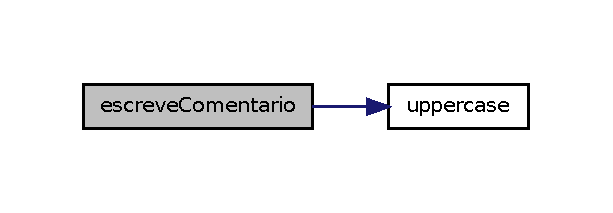
\includegraphics[width=294pt]{resposta_8c_a2b6f397b0bfae5590b292d282513c54b_cgraph}
\end{center}
\end{figure}




Este é o diagrama das funções que utilizam esta função:
\nopagebreak
\begin{figure}[H]
\begin{center}
\leavevmode
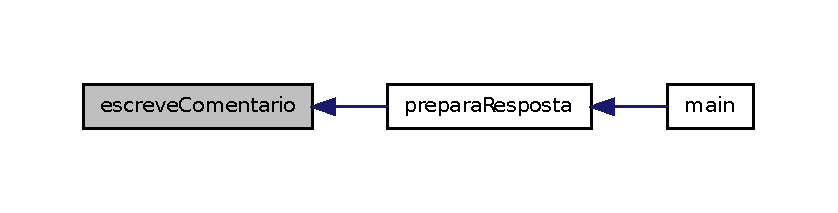
\includegraphics[width=400pt]{resposta_8c_a2b6f397b0bfae5590b292d282513c54b_icgraph}
\end{center}
\end{figure}


\hypertarget{resposta_8c_a6c04d45a3b24b43c86d50889bde25d67}{
\index{resposta.c@{resposta.c}!infoDisciplina@{infoDisciplina}}
\index{infoDisciplina@{infoDisciplina}!resposta.c@{resposta.c}}
\subsubsection[{infoDisciplina}]{\setlength{\rightskip}{0pt plus 5cm}char$\ast$ infoDisciplina (
\begin{DoxyParamCaption}
\item[{char $\ast$}]{disc}
\end{DoxyParamCaption}
)}}
\label{resposta_8c_a6c04d45a3b24b43c86d50889bde25d67}
Função que retorna ao cliente todas as informações de uma disciplina requisitada, se essa existir.

disc -\/ a sigla da disciplina

string com todas as informações sobre a disciplina 

Definição na linha 331 do arquivo resposta.c.



Este é o diagrama das funções utilizadas por esta função:
\nopagebreak
\begin{figure}[H]
\begin{center}
\leavevmode
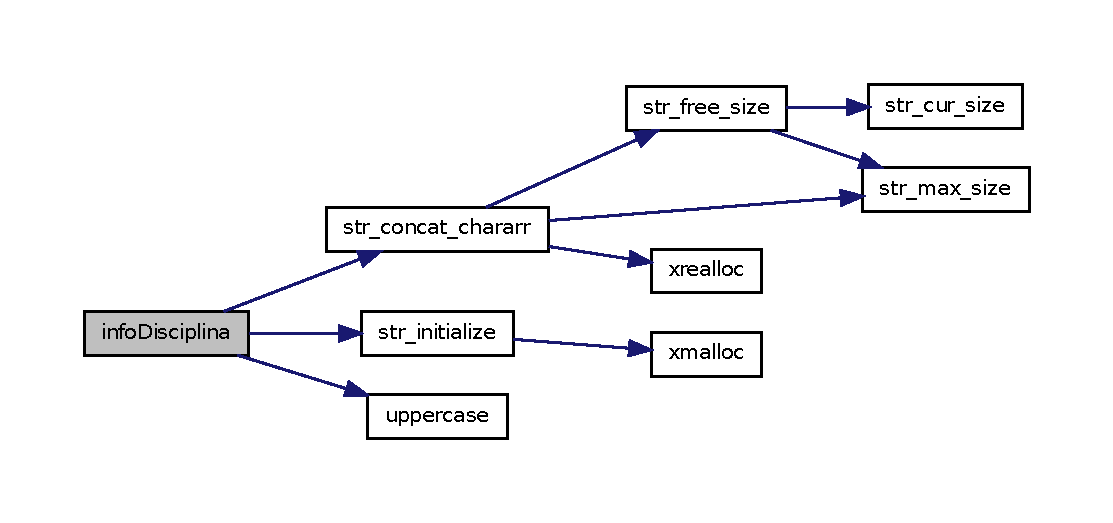
\includegraphics[width=400pt]{resposta_8c_a6c04d45a3b24b43c86d50889bde25d67_cgraph}
\end{center}
\end{figure}




Este é o diagrama das funções que utilizam esta função:
\nopagebreak
\begin{figure}[H]
\begin{center}
\leavevmode
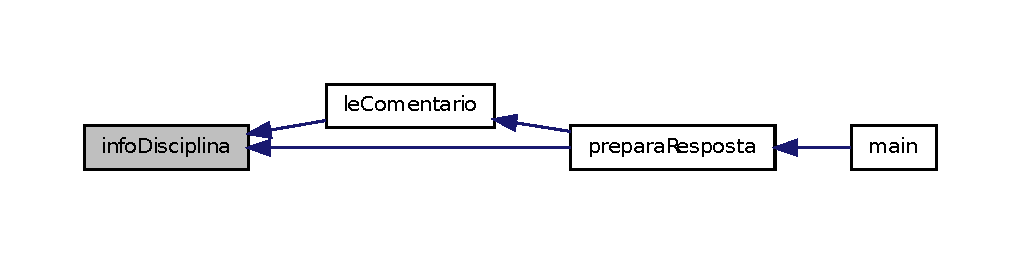
\includegraphics[width=400pt]{resposta_8c_a6c04d45a3b24b43c86d50889bde25d67_icgraph}
\end{center}
\end{figure}


\hypertarget{resposta_8c_aae0e9c217f1ede36bbf9821b36bba3f9}{
\index{resposta.c@{resposta.c}!infoDisciplinas@{infoDisciplinas}}
\index{infoDisciplinas@{infoDisciplinas}!resposta.c@{resposta.c}}
\subsubsection[{infoDisciplinas}]{\setlength{\rightskip}{0pt plus 5cm}char$\ast$ infoDisciplinas (
\begin{DoxyParamCaption}
{}
\end{DoxyParamCaption}
)}}
\label{resposta_8c_aae0e9c217f1ede36bbf9821b36bba3f9}
Função que retorna as informações de todas as disciplinas cadastradas no servidor.

Uma string com as informações de todas as disciplinas 

Definição na linha 258 do arquivo resposta.c.



Este é o diagrama das funções utilizadas por esta função:
\nopagebreak
\begin{figure}[H]
\begin{center}
\leavevmode
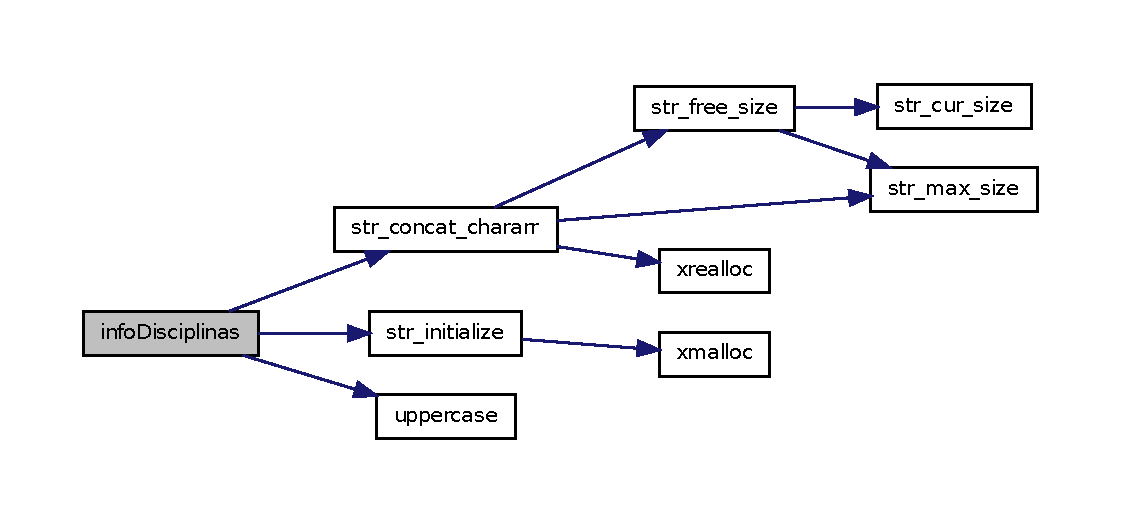
\includegraphics[width=400pt]{resposta_8c_aae0e9c217f1ede36bbf9821b36bba3f9_cgraph}
\end{center}
\end{figure}




Este é o diagrama das funções que utilizam esta função:
\nopagebreak
\begin{figure}[H]
\begin{center}
\leavevmode
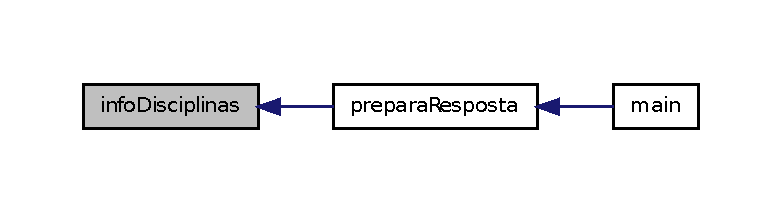
\includegraphics[width=376pt]{resposta_8c_aae0e9c217f1ede36bbf9821b36bba3f9_icgraph}
\end{center}
\end{figure}


\hypertarget{resposta_8c_a2a098bc71f2a19dd74318fd778676979}{
\index{resposta.c@{resposta.c}!leComentario@{leComentario}}
\index{leComentario@{leComentario}!resposta.c@{resposta.c}}
\subsubsection[{leComentario}]{\setlength{\rightskip}{0pt plus 5cm}char$\ast$ leComentario (
\begin{DoxyParamCaption}
\item[{char $\ast$}]{disc}
\end{DoxyParamCaption}
)}}
\label{resposta_8c_a2a098bc71f2a19dd74318fd778676979}
Função que le os comentários escritos para uma certa disciplina, retornando-\/os.

disc -\/ a sigla da disciplina

uma string com todos os comentários da disciplina 

Definição na linha 71 do arquivo resposta.c.



Este é o diagrama das funções utilizadas por esta função:
\nopagebreak
\begin{figure}[H]
\begin{center}
\leavevmode
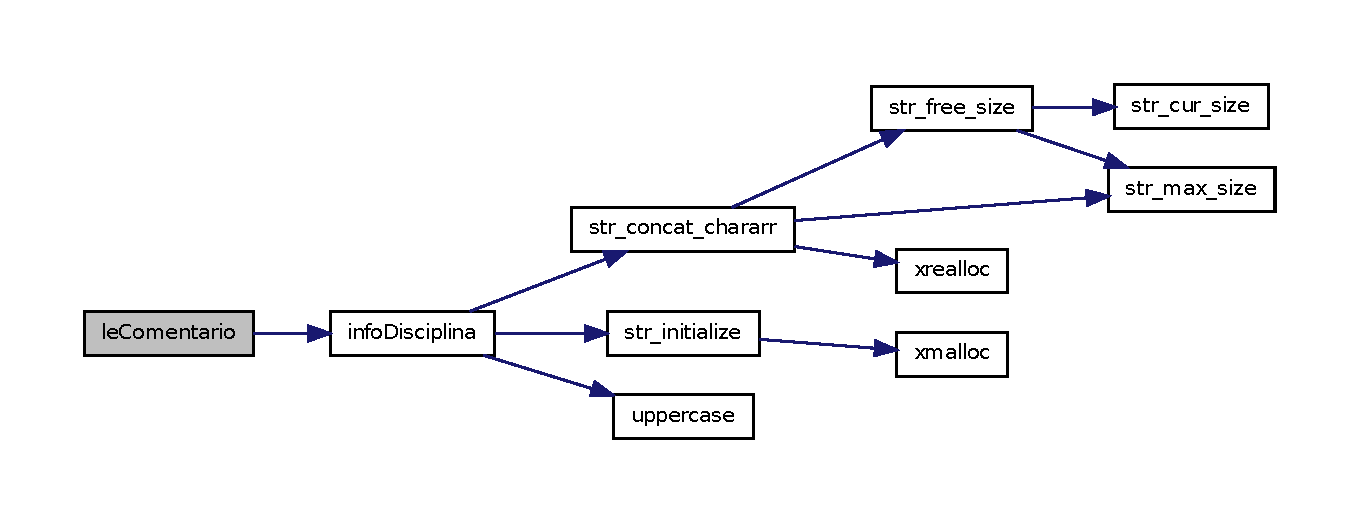
\includegraphics[width=400pt]{resposta_8c_a2a098bc71f2a19dd74318fd778676979_cgraph}
\end{center}
\end{figure}




Este é o diagrama das funções que utilizam esta função:
\nopagebreak
\begin{figure}[H]
\begin{center}
\leavevmode
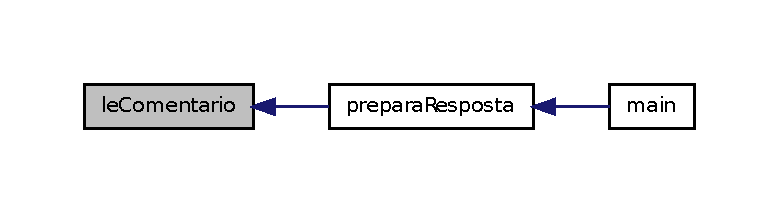
\includegraphics[width=374pt]{resposta_8c_a2a098bc71f2a19dd74318fd778676979_icgraph}
\end{center}
\end{figure}


\hypertarget{resposta_8c_adca402fde30bac4845d32a7dd4e6160a}{
\index{resposta.c@{resposta.c}!listaDisciplinas@{listaDisciplinas}}
\index{listaDisciplinas@{listaDisciplinas}!resposta.c@{resposta.c}}
\subsubsection[{listaDisciplinas}]{\setlength{\rightskip}{0pt plus 5cm}char$\ast$ listaDisciplinas (
\begin{DoxyParamCaption}
{}
\end{DoxyParamCaption}
)}}
\label{resposta_8c_adca402fde30bac4845d32a7dd4e6160a}
Função que lista todas as disciplinas cadastradas no servidor.

string com as siglas e nomes das disciplinas cadastradas. 

Definição na linha 140 do arquivo resposta.c.



Este é o diagrama das funções utilizadas por esta função:
\nopagebreak
\begin{figure}[H]
\begin{center}
\leavevmode
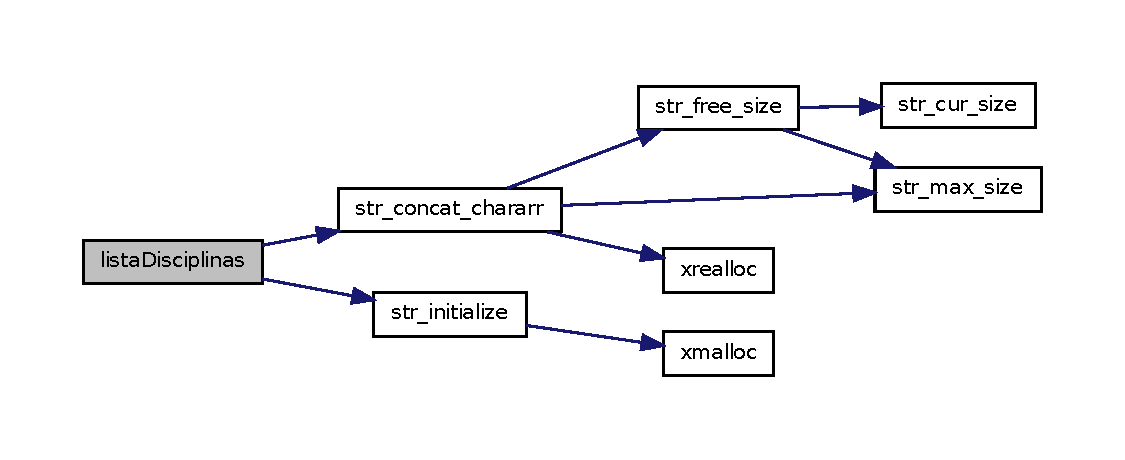
\includegraphics[width=400pt]{resposta_8c_adca402fde30bac4845d32a7dd4e6160a_cgraph}
\end{center}
\end{figure}




Este é o diagrama das funções que utilizam esta função:
\nopagebreak
\begin{figure}[H]
\begin{center}
\leavevmode
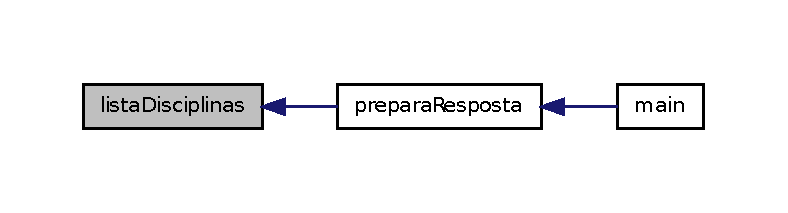
\includegraphics[width=378pt]{resposta_8c_adca402fde30bac4845d32a7dd4e6160a_icgraph}
\end{center}
\end{figure}


\hypertarget{resposta_8c_a9bb7e31e6340d62b3afb839655847563}{
\index{resposta.c@{resposta.c}!preparaResposta@{preparaResposta}}
\index{preparaResposta@{preparaResposta}!resposta.c@{resposta.c}}
\subsubsection[{preparaResposta}]{\setlength{\rightskip}{0pt plus 5cm}char$\ast$ preparaResposta (
\begin{DoxyParamCaption}
\item[{char $\ast$}]{buf}
\end{DoxyParamCaption}
)}}
\label{resposta_8c_a9bb7e31e6340d62b3afb839655847563}
Função que recebe um parâmetro do cliente e, a partir disso, executa as rotinas apropriadas, preparando a resposta adequada a ser enviada ao cliente.

buf -\/ string recebida pelo cliente

string com a resposta esperada pelo cliente 

Definição na linha 19 do arquivo resposta.c.



Este é o diagrama das funções utilizadas por esta função:
\nopagebreak
\begin{figure}[H]
\begin{center}
\leavevmode
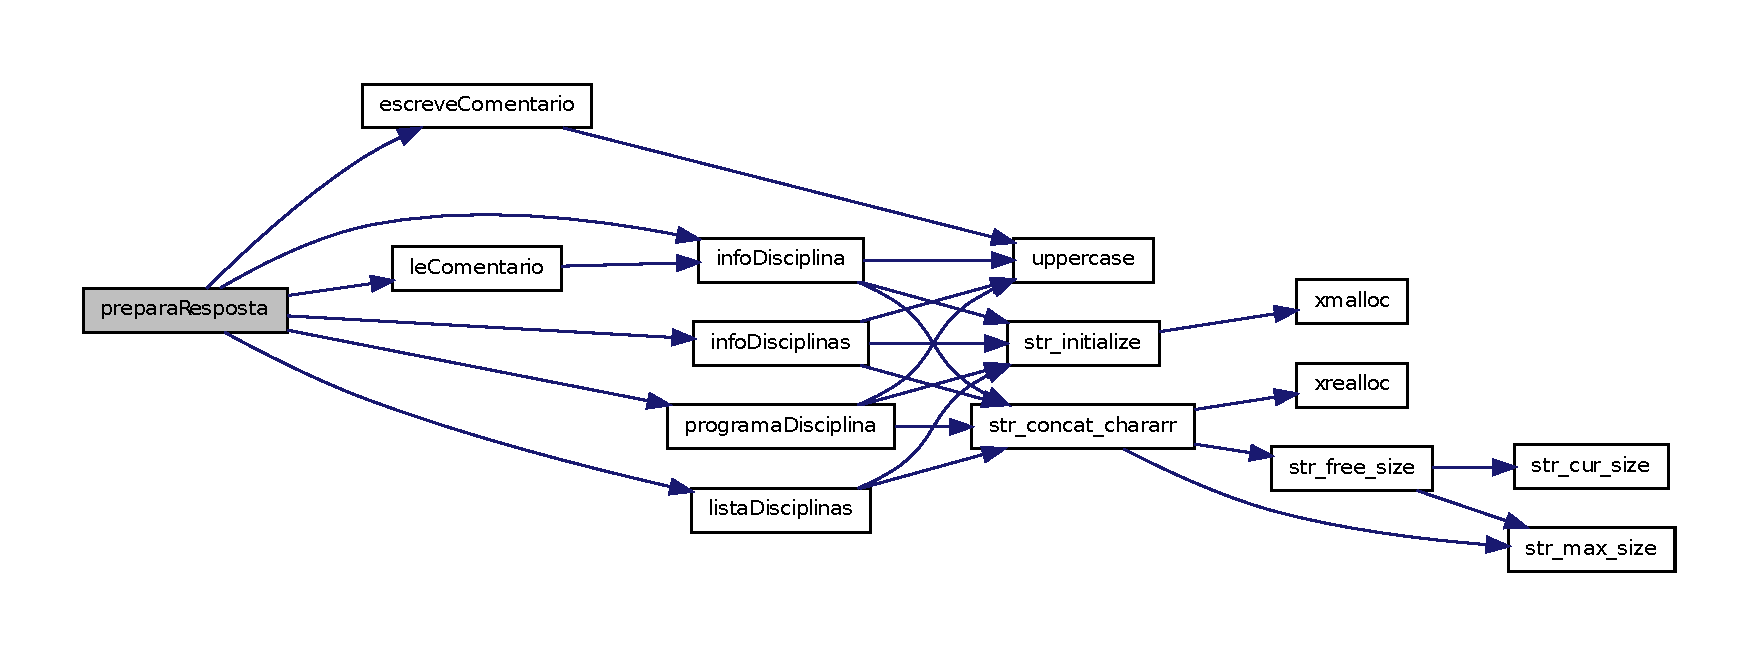
\includegraphics[width=400pt]{resposta_8c_a9bb7e31e6340d62b3afb839655847563_cgraph}
\end{center}
\end{figure}




Este é o diagrama das funções que utilizam esta função:
\nopagebreak
\begin{figure}[H]
\begin{center}
\leavevmode
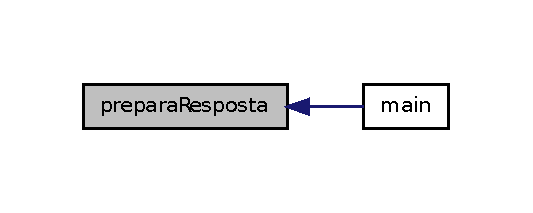
\includegraphics[width=256pt]{resposta_8c_a9bb7e31e6340d62b3afb839655847563_icgraph}
\end{center}
\end{figure}


\hypertarget{resposta_8c_ae53e5d927eddd073efa7dd3777c222c2}{
\index{resposta.c@{resposta.c}!programaDisciplina@{programaDisciplina}}
\index{programaDisciplina@{programaDisciplina}!resposta.c@{resposta.c}}
\subsubsection[{programaDisciplina}]{\setlength{\rightskip}{0pt plus 5cm}char$\ast$ programaDisciplina (
\begin{DoxyParamCaption}
\item[{char $\ast$}]{disc}
\end{DoxyParamCaption}
)}}
\label{resposta_8c_ae53e5d927eddd073efa7dd3777c222c2}
Função que retorna ao cliente o programa de uma determinada disciplina, se essa existir.

disc -\/ a sigla da disciplina requisitada

string com o programa da disciplina 

Definição na linha 186 do arquivo resposta.c.



Este é o diagrama das funções utilizadas por esta função:
\nopagebreak
\begin{figure}[H]
\begin{center}
\leavevmode
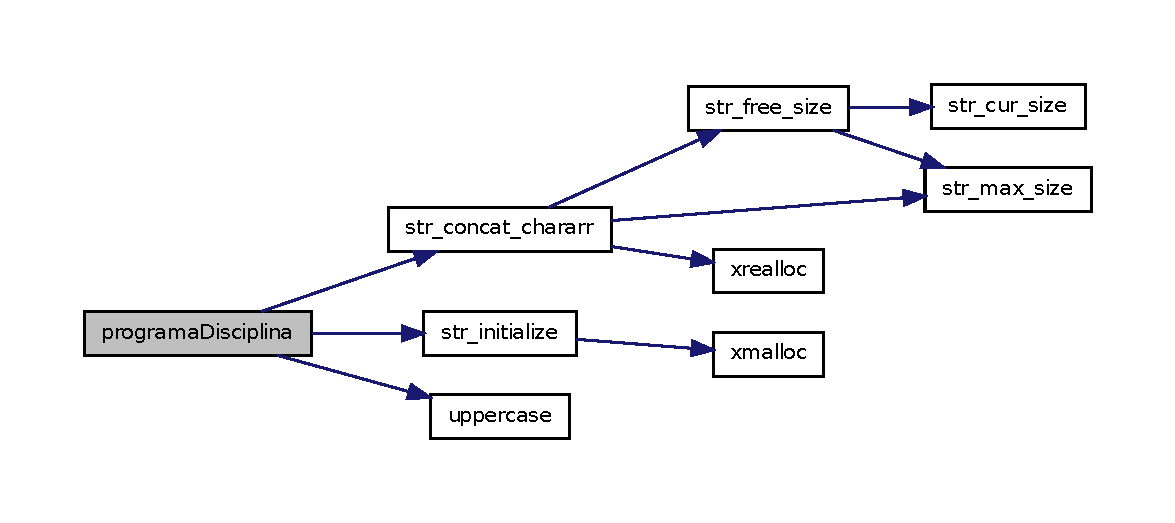
\includegraphics[width=400pt]{resposta_8c_ae53e5d927eddd073efa7dd3777c222c2_cgraph}
\end{center}
\end{figure}




Este é o diagrama das funções que utilizam esta função:
\nopagebreak
\begin{figure}[H]
\begin{center}
\leavevmode
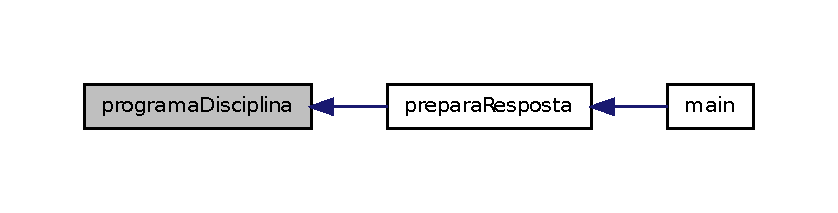
\includegraphics[width=400pt]{resposta_8c_ae53e5d927eddd073efa7dd3777c222c2_icgraph}
\end{center}
\end{figure}


\hypertarget{resposta_8c_aaf2c986b7320373a463f607a67c07365}{
\index{resposta.c@{resposta.c}!uppercase@{uppercase}}
\index{uppercase@{uppercase}!resposta.c@{resposta.c}}
\subsubsection[{uppercase}]{\setlength{\rightskip}{0pt plus 5cm}void uppercase (
\begin{DoxyParamCaption}
\item[{char $\ast$}]{sPtr}
\end{DoxyParamCaption}
)}}
\label{resposta_8c_aaf2c986b7320373a463f607a67c07365}
Função auxiliar que converte todos os caracteres de uma string para letra maiúscula.

sPtr -\/ String a ser padronizada 

Definição na linha 391 do arquivo resposta.c.



Este é o diagrama das funções que utilizam esta função:
\nopagebreak
\begin{figure}[H]
\begin{center}
\leavevmode
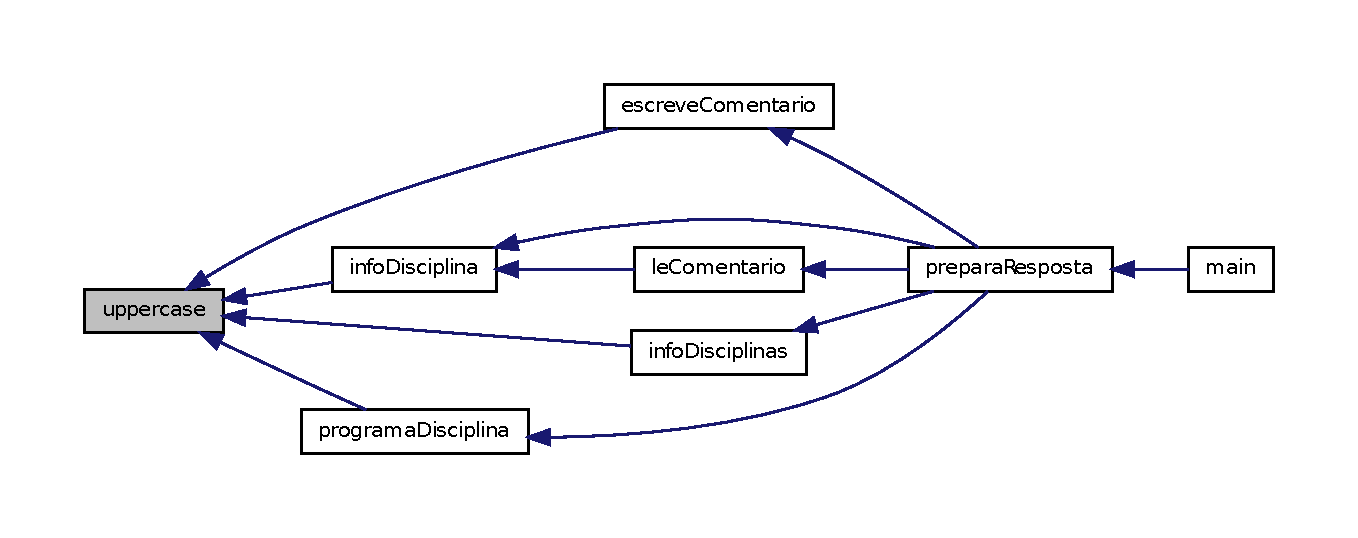
\includegraphics[width=400pt]{resposta_8c_aaf2c986b7320373a463f607a67c07365_icgraph}
\end{center}
\end{figure}



\hypertarget{resposta_8h}{
\section{Referência do Arquivo resposta.h}
\label{resposta_8h}\index{resposta.h@{resposta.h}}
}
{\ttfamily \#include \char`\"{}str.h\char`\"{}}\par
Gráfico de dependência de inclusões para resposta.h:
\nopagebreak
\begin{figure}[H]
\begin{center}
\leavevmode
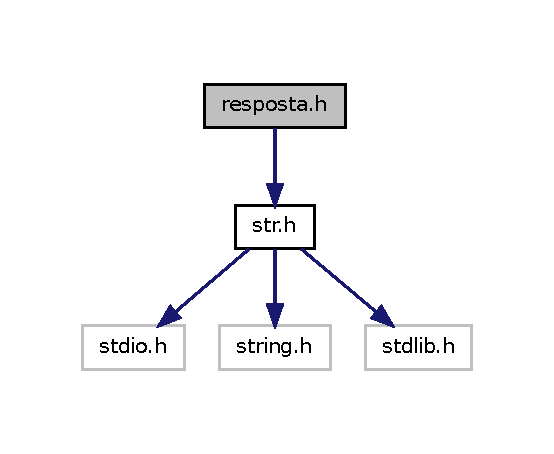
\includegraphics[width=266pt]{resposta_8h__incl}
\end{center}
\end{figure}
Este grafo mostra quais arquivos estão direta ou indiretamente relacionados com este arquivo:
\nopagebreak
\begin{figure}[H]
\begin{center}
\leavevmode
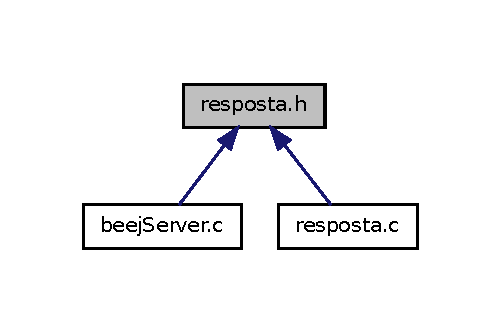
\includegraphics[width=240pt]{resposta_8h__dep__incl}
\end{center}
\end{figure}
\subsection*{Funções}
\begin{DoxyCompactItemize}
\item 
char $\ast$ \hyperlink{resposta_8h_a9bb7e31e6340d62b3afb839655847563}{preparaResposta} (char $\ast$buf)
\item 
char $\ast$ \hyperlink{resposta_8h_adca402fde30bac4845d32a7dd4e6160a}{listaDisciplinas} ()
\item 
char $\ast$ \hyperlink{resposta_8h_aae0e9c217f1ede36bbf9821b36bba3f9}{infoDisciplinas} ()
\item 
char $\ast$ \hyperlink{resposta_8h_a6c04d45a3b24b43c86d50889bde25d67}{infoDisciplina} (char $\ast$disc)
\item 
char $\ast$ \hyperlink{resposta_8h_ae53e5d927eddd073efa7dd3777c222c2}{programaDisciplina} (char $\ast$disc)
\item 
char $\ast$ \hyperlink{resposta_8h_a2b6f397b0bfae5590b292d282513c54b}{escreveComentario} (char $\ast$disc, char $\ast$comentario)
\item 
char $\ast$ \hyperlink{resposta_8h_a2a098bc71f2a19dd74318fd778676979}{leComentario} (char $\ast$disc)
\item 
void \hyperlink{resposta_8h_aaf2c986b7320373a463f607a67c07365}{uppercase} (char $\ast$sPtr)
\item 
char $\ast$ \hyperlink{resposta_8h_aedc478ab50fc92caf2f60a72e72369d4}{retiraSubstring} (char $\ast$\hyperlink{structstr}{str}, int lenstr, char $\ast$sub, int lensub)
\item 
int \hyperlink{resposta_8h_a162a0a0cfa88262241cb9d881c6f505b}{verificaSubstring} (char $\ast$\hyperlink{structstr}{str}, int lenstr, char $\ast$sub, int lensub)
\end{DoxyCompactItemize}


\subsection{Funções}
\hypertarget{resposta_8h_a2b6f397b0bfae5590b292d282513c54b}{
\index{resposta.h@{resposta.h}!escreveComentario@{escreveComentario}}
\index{escreveComentario@{escreveComentario}!resposta.h@{resposta.h}}
\subsubsection[{escreveComentario}]{\setlength{\rightskip}{0pt plus 5cm}char$\ast$ escreveComentario (
\begin{DoxyParamCaption}
\item[{char $\ast$}]{disc, }
\item[{char $\ast$}]{comentario}
\end{DoxyParamCaption}
)}}
\label{resposta_8h_a2b6f397b0bfae5590b292d282513c54b}
Função que escreve um comentário enviado pelo cliente para o servidor. A escrita do comentário se dá na disciplina passada pelo cliente, se existir.

disc -\/ sigla da disciplina  comentario -\/ comentário a ser escrito

String com uma mensagem de sucesso, caso a escrita seja bem sucedida. 

Definição na linha 111 do arquivo resposta.c.



Este é o diagrama das funções utilizadas por esta função:
\nopagebreak
\begin{figure}[H]
\begin{center}
\leavevmode
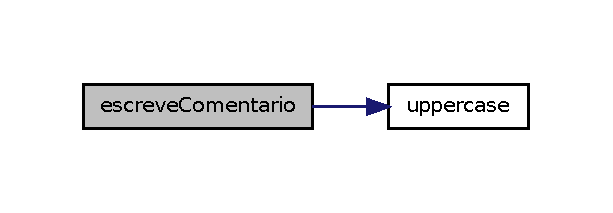
\includegraphics[width=294pt]{resposta_8h_a2b6f397b0bfae5590b292d282513c54b_cgraph}
\end{center}
\end{figure}




Este é o diagrama das funções que utilizam esta função:
\nopagebreak
\begin{figure}[H]
\begin{center}
\leavevmode
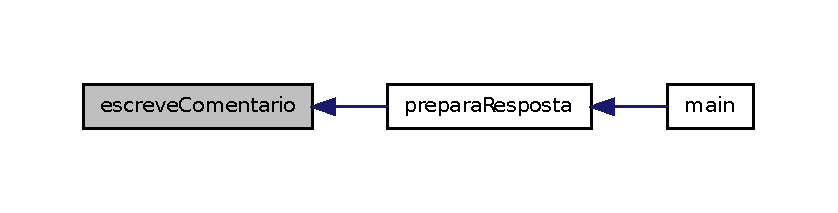
\includegraphics[width=400pt]{resposta_8h_a2b6f397b0bfae5590b292d282513c54b_icgraph}
\end{center}
\end{figure}


\hypertarget{resposta_8h_a6c04d45a3b24b43c86d50889bde25d67}{
\index{resposta.h@{resposta.h}!infoDisciplina@{infoDisciplina}}
\index{infoDisciplina@{infoDisciplina}!resposta.h@{resposta.h}}
\subsubsection[{infoDisciplina}]{\setlength{\rightskip}{0pt plus 5cm}char$\ast$ infoDisciplina (
\begin{DoxyParamCaption}
\item[{char $\ast$}]{disc}
\end{DoxyParamCaption}
)}}
\label{resposta_8h_a6c04d45a3b24b43c86d50889bde25d67}
Função que retorna ao cliente todas as informações de uma disciplina requisitada, se essa existir.

disc -\/ a sigla da disciplina

string com todas as informações sobre a disciplina 

Definição na linha 331 do arquivo resposta.c.



Este é o diagrama das funções utilizadas por esta função:
\nopagebreak
\begin{figure}[H]
\begin{center}
\leavevmode
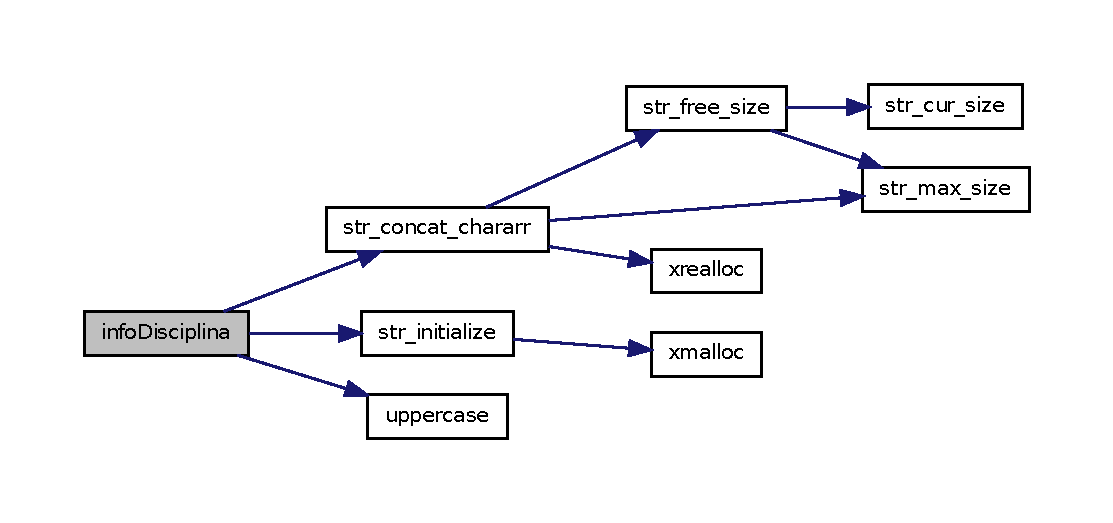
\includegraphics[width=400pt]{resposta_8h_a6c04d45a3b24b43c86d50889bde25d67_cgraph}
\end{center}
\end{figure}




Este é o diagrama das funções que utilizam esta função:
\nopagebreak
\begin{figure}[H]
\begin{center}
\leavevmode
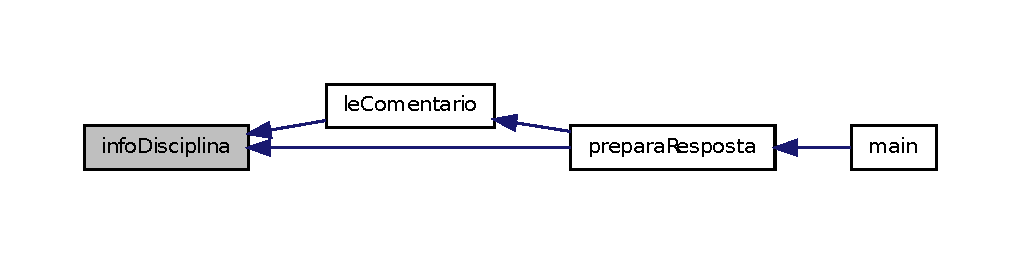
\includegraphics[width=400pt]{resposta_8h_a6c04d45a3b24b43c86d50889bde25d67_icgraph}
\end{center}
\end{figure}


\hypertarget{resposta_8h_aae0e9c217f1ede36bbf9821b36bba3f9}{
\index{resposta.h@{resposta.h}!infoDisciplinas@{infoDisciplinas}}
\index{infoDisciplinas@{infoDisciplinas}!resposta.h@{resposta.h}}
\subsubsection[{infoDisciplinas}]{\setlength{\rightskip}{0pt plus 5cm}char$\ast$ infoDisciplinas (
\begin{DoxyParamCaption}
{}
\end{DoxyParamCaption}
)}}
\label{resposta_8h_aae0e9c217f1ede36bbf9821b36bba3f9}
Função que retorna as informações de todas as disciplinas cadastradas no servidor.

Uma string com as informações de todas as disciplinas 

Definição na linha 258 do arquivo resposta.c.



Este é o diagrama das funções utilizadas por esta função:
\nopagebreak
\begin{figure}[H]
\begin{center}
\leavevmode
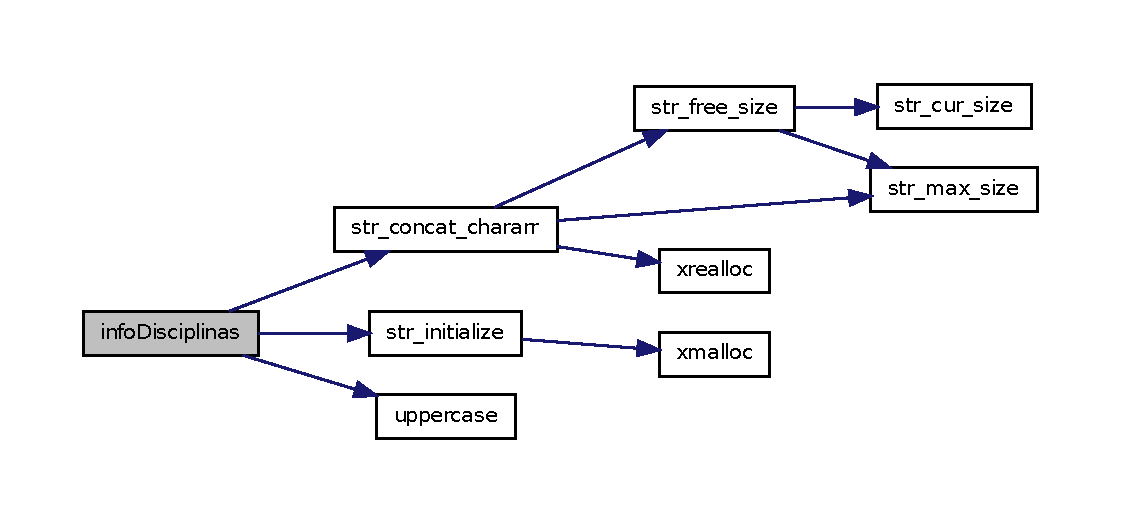
\includegraphics[width=400pt]{resposta_8h_aae0e9c217f1ede36bbf9821b36bba3f9_cgraph}
\end{center}
\end{figure}




Este é o diagrama das funções que utilizam esta função:
\nopagebreak
\begin{figure}[H]
\begin{center}
\leavevmode
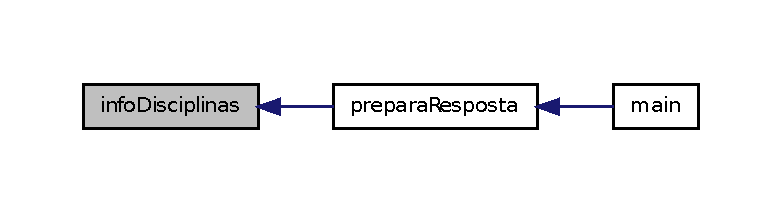
\includegraphics[width=376pt]{resposta_8h_aae0e9c217f1ede36bbf9821b36bba3f9_icgraph}
\end{center}
\end{figure}


\hypertarget{resposta_8h_a2a098bc71f2a19dd74318fd778676979}{
\index{resposta.h@{resposta.h}!leComentario@{leComentario}}
\index{leComentario@{leComentario}!resposta.h@{resposta.h}}
\subsubsection[{leComentario}]{\setlength{\rightskip}{0pt plus 5cm}char$\ast$ leComentario (
\begin{DoxyParamCaption}
\item[{char $\ast$}]{disc}
\end{DoxyParamCaption}
)}}
\label{resposta_8h_a2a098bc71f2a19dd74318fd778676979}
Função que le os comentários escritos para uma certa disciplina, retornando-\/os.

disc -\/ a sigla da disciplina

uma string com todos os comentários da disciplina 

Definição na linha 71 do arquivo resposta.c.



Este é o diagrama das funções utilizadas por esta função:
\nopagebreak
\begin{figure}[H]
\begin{center}
\leavevmode
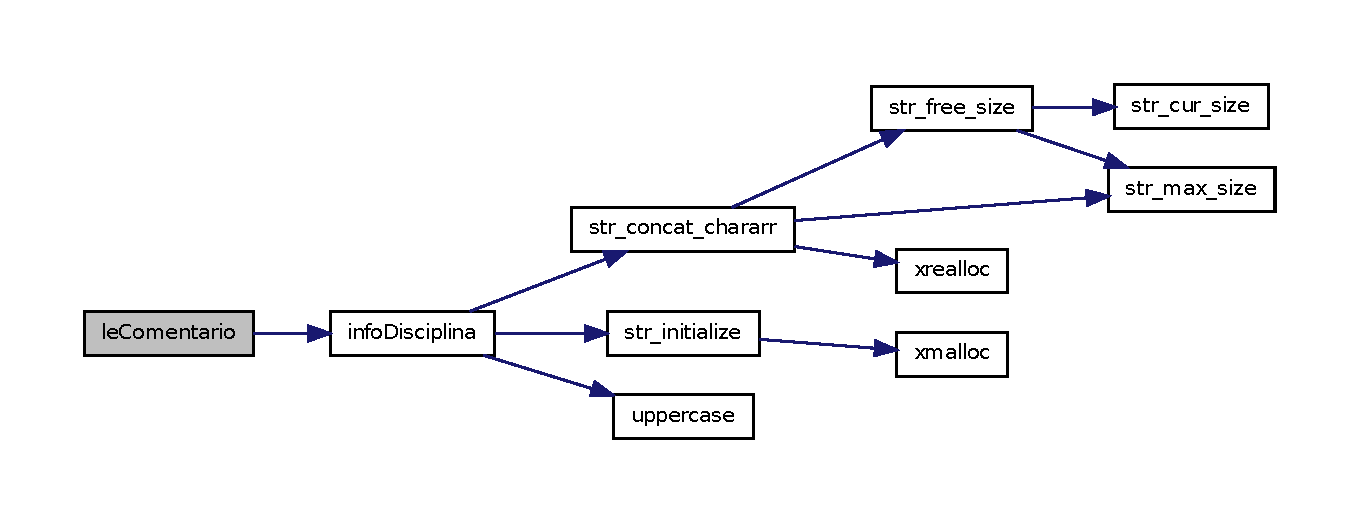
\includegraphics[width=400pt]{resposta_8h_a2a098bc71f2a19dd74318fd778676979_cgraph}
\end{center}
\end{figure}




Este é o diagrama das funções que utilizam esta função:
\nopagebreak
\begin{figure}[H]
\begin{center}
\leavevmode
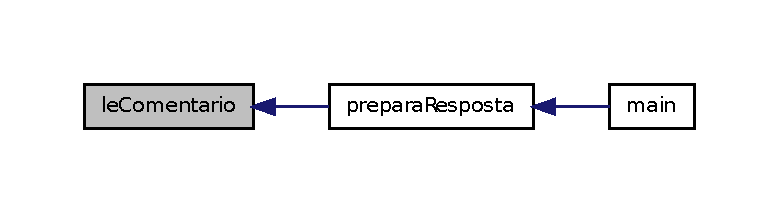
\includegraphics[width=374pt]{resposta_8h_a2a098bc71f2a19dd74318fd778676979_icgraph}
\end{center}
\end{figure}


\hypertarget{resposta_8h_adca402fde30bac4845d32a7dd4e6160a}{
\index{resposta.h@{resposta.h}!listaDisciplinas@{listaDisciplinas}}
\index{listaDisciplinas@{listaDisciplinas}!resposta.h@{resposta.h}}
\subsubsection[{listaDisciplinas}]{\setlength{\rightskip}{0pt plus 5cm}char$\ast$ listaDisciplinas (
\begin{DoxyParamCaption}
{}
\end{DoxyParamCaption}
)}}
\label{resposta_8h_adca402fde30bac4845d32a7dd4e6160a}
Função que lista todas as disciplinas cadastradas no servidor.

string com as siglas e nomes das disciplinas cadastradas. 

Definição na linha 140 do arquivo resposta.c.



Este é o diagrama das funções utilizadas por esta função:
\nopagebreak
\begin{figure}[H]
\begin{center}
\leavevmode
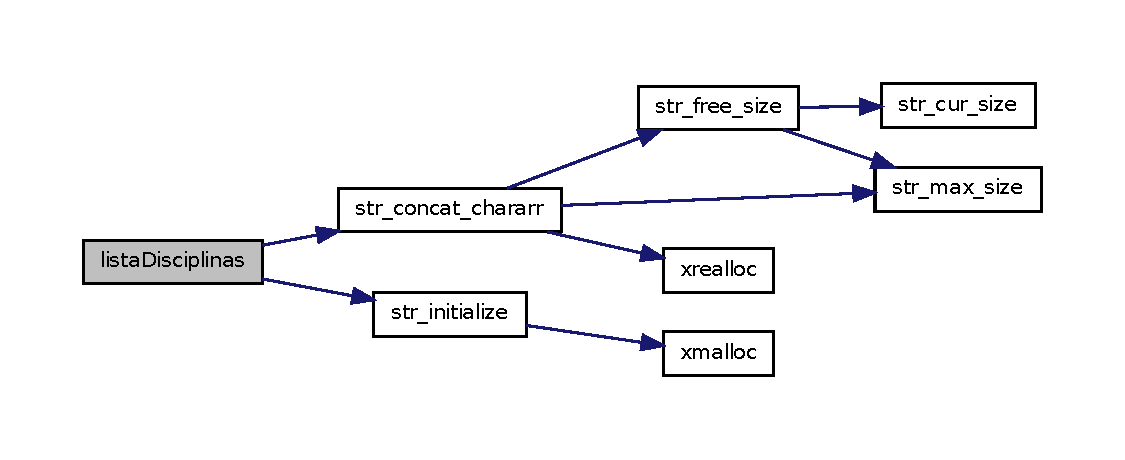
\includegraphics[width=400pt]{resposta_8h_adca402fde30bac4845d32a7dd4e6160a_cgraph}
\end{center}
\end{figure}




Este é o diagrama das funções que utilizam esta função:
\nopagebreak
\begin{figure}[H]
\begin{center}
\leavevmode
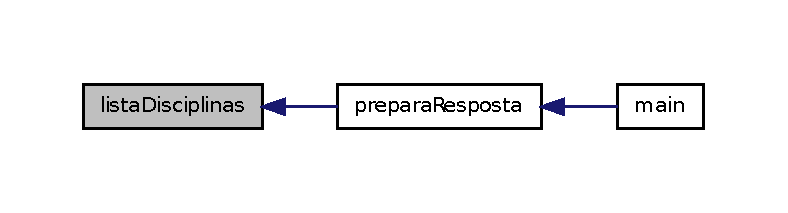
\includegraphics[width=378pt]{resposta_8h_adca402fde30bac4845d32a7dd4e6160a_icgraph}
\end{center}
\end{figure}


\hypertarget{resposta_8h_a9bb7e31e6340d62b3afb839655847563}{
\index{resposta.h@{resposta.h}!preparaResposta@{preparaResposta}}
\index{preparaResposta@{preparaResposta}!resposta.h@{resposta.h}}
\subsubsection[{preparaResposta}]{\setlength{\rightskip}{0pt plus 5cm}char$\ast$ preparaResposta (
\begin{DoxyParamCaption}
\item[{char $\ast$}]{buf}
\end{DoxyParamCaption}
)}}
\label{resposta_8h_a9bb7e31e6340d62b3afb839655847563}
Função que recebe um parâmetro do cliente e, a partir disso, executa as rotinas apropriadas, preparando a resposta adequada a ser enviada ao cliente.

buf -\/ string recebida pelo cliente

string com a resposta esperada pelo cliente 

Definição na linha 19 do arquivo resposta.c.



Este é o diagrama das funções utilizadas por esta função:
\nopagebreak
\begin{figure}[H]
\begin{center}
\leavevmode
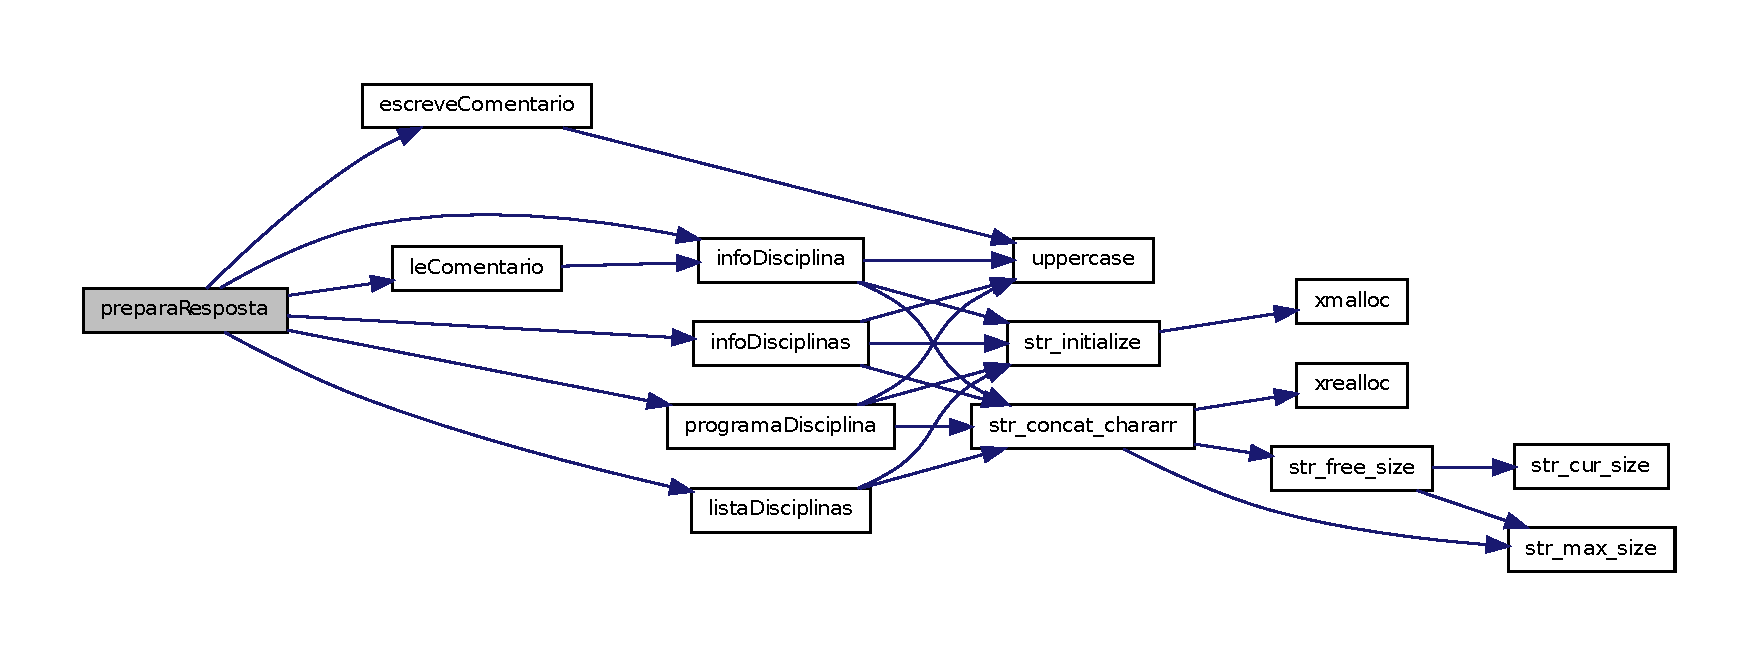
\includegraphics[width=400pt]{resposta_8h_a9bb7e31e6340d62b3afb839655847563_cgraph}
\end{center}
\end{figure}




Este é o diagrama das funções que utilizam esta função:
\nopagebreak
\begin{figure}[H]
\begin{center}
\leavevmode
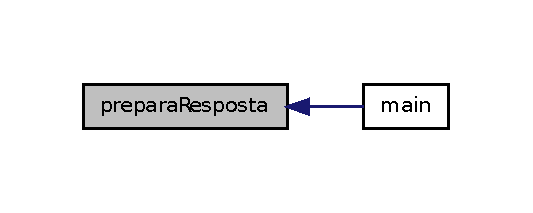
\includegraphics[width=256pt]{resposta_8h_a9bb7e31e6340d62b3afb839655847563_icgraph}
\end{center}
\end{figure}


\hypertarget{resposta_8h_ae53e5d927eddd073efa7dd3777c222c2}{
\index{resposta.h@{resposta.h}!programaDisciplina@{programaDisciplina}}
\index{programaDisciplina@{programaDisciplina}!resposta.h@{resposta.h}}
\subsubsection[{programaDisciplina}]{\setlength{\rightskip}{0pt plus 5cm}char$\ast$ programaDisciplina (
\begin{DoxyParamCaption}
\item[{char $\ast$}]{disc}
\end{DoxyParamCaption}
)}}
\label{resposta_8h_ae53e5d927eddd073efa7dd3777c222c2}
Função que retorna ao cliente o programa de uma determinada disciplina, se essa existir.

disc -\/ a sigla da disciplina requisitada

string com o programa da disciplina 

Definição na linha 186 do arquivo resposta.c.



Este é o diagrama das funções utilizadas por esta função:
\nopagebreak
\begin{figure}[H]
\begin{center}
\leavevmode
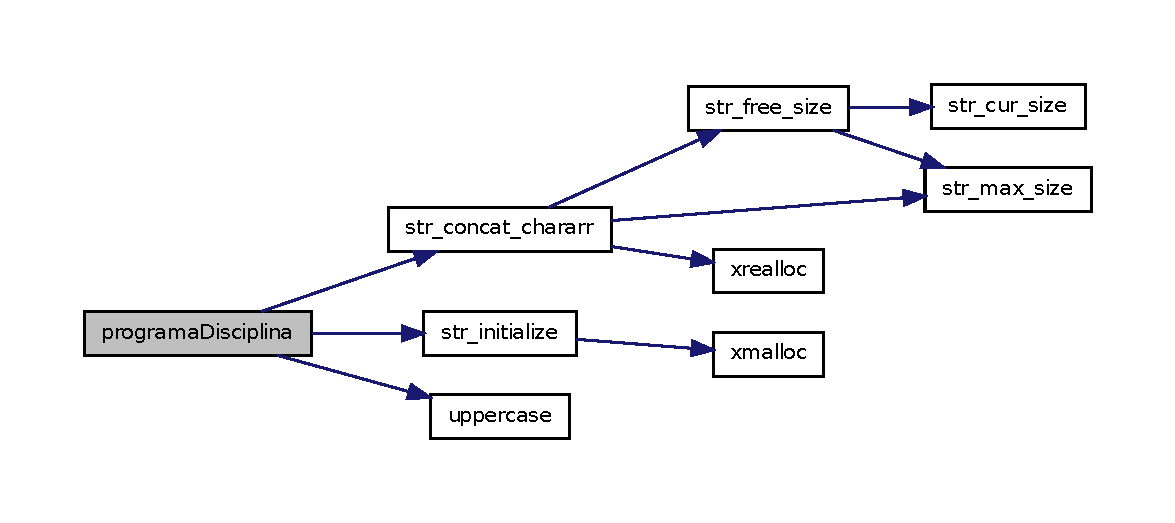
\includegraphics[width=400pt]{resposta_8h_ae53e5d927eddd073efa7dd3777c222c2_cgraph}
\end{center}
\end{figure}




Este é o diagrama das funções que utilizam esta função:
\nopagebreak
\begin{figure}[H]
\begin{center}
\leavevmode
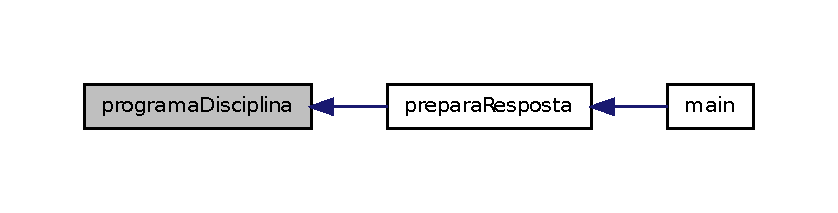
\includegraphics[width=400pt]{resposta_8h_ae53e5d927eddd073efa7dd3777c222c2_icgraph}
\end{center}
\end{figure}


\hypertarget{resposta_8h_aedc478ab50fc92caf2f60a72e72369d4}{
\index{resposta.h@{resposta.h}!retiraSubstring@{retiraSubstring}}
\index{retiraSubstring@{retiraSubstring}!resposta.h@{resposta.h}}
\subsubsection[{retiraSubstring}]{\setlength{\rightskip}{0pt plus 5cm}char$\ast$ retiraSubstring (
\begin{DoxyParamCaption}
\item[{char $\ast$}]{str, }
\item[{int}]{lenstr, }
\item[{char $\ast$}]{sub, }
\item[{int}]{lensub}
\end{DoxyParamCaption}
)}}
\label{resposta_8h_aedc478ab50fc92caf2f60a72e72369d4}
\hypertarget{resposta_8h_aaf2c986b7320373a463f607a67c07365}{
\index{resposta.h@{resposta.h}!uppercase@{uppercase}}
\index{uppercase@{uppercase}!resposta.h@{resposta.h}}
\subsubsection[{uppercase}]{\setlength{\rightskip}{0pt plus 5cm}void uppercase (
\begin{DoxyParamCaption}
\item[{char $\ast$}]{sPtr}
\end{DoxyParamCaption}
)}}
\label{resposta_8h_aaf2c986b7320373a463f607a67c07365}
Função auxiliar que converte todos os caracteres de uma string para letra maiúscula.

sPtr -\/ String a ser padronizada 

Definição na linha 391 do arquivo resposta.c.



Este é o diagrama das funções que utilizam esta função:
\nopagebreak
\begin{figure}[H]
\begin{center}
\leavevmode
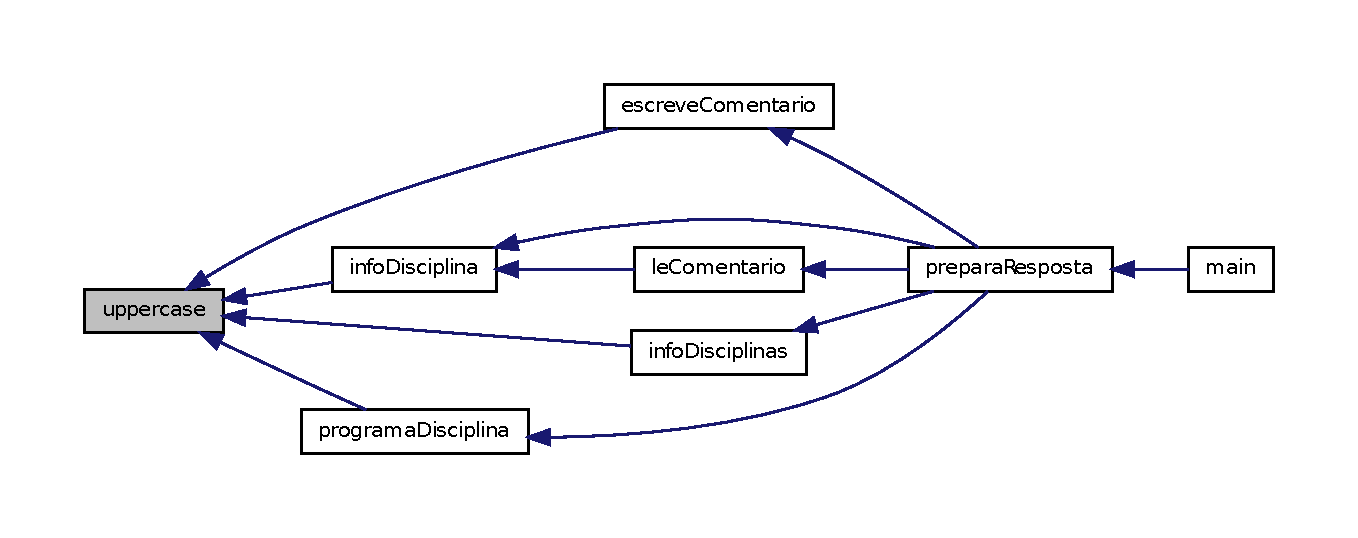
\includegraphics[width=400pt]{resposta_8h_aaf2c986b7320373a463f607a67c07365_icgraph}
\end{center}
\end{figure}


\hypertarget{resposta_8h_a162a0a0cfa88262241cb9d881c6f505b}{
\index{resposta.h@{resposta.h}!verificaSubstring@{verificaSubstring}}
\index{verificaSubstring@{verificaSubstring}!resposta.h@{resposta.h}}
\subsubsection[{verificaSubstring}]{\setlength{\rightskip}{0pt plus 5cm}int verificaSubstring (
\begin{DoxyParamCaption}
\item[{char $\ast$}]{str, }
\item[{int}]{lenstr, }
\item[{char $\ast$}]{sub, }
\item[{int}]{lensub}
\end{DoxyParamCaption}
)}}
\label{resposta_8h_a162a0a0cfa88262241cb9d881c6f505b}

\hypertarget{str_8c}{
\section{Referência do Arquivo str.c}
\label{str_8c}\index{str.c@{str.c}}
}
{\ttfamily \#include \char`\"{}mm.h\char`\"{}}\par
{\ttfamily \#include \char`\"{}str.h\char`\"{}}\par
Gráfico de dependência de inclusões para str.c:
\nopagebreak
\begin{figure}[H]
\begin{center}
\leavevmode
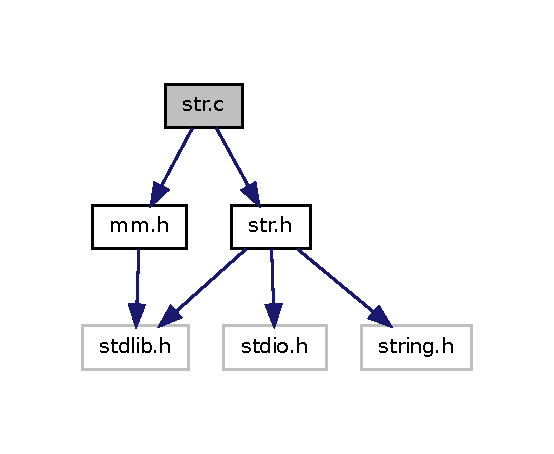
\includegraphics[width=266pt]{str_8c__incl}
\end{center}
\end{figure}
\subsection*{Funções}
\begin{DoxyCompactItemize}
\item 
\hyperlink{structstr}{string} \hyperlink{str_8c_a43e9efab3e78f169462b9f842c827fba}{str\_\-initialize} (size\_\-t size)
\item 
int \hyperlink{str_8c_a4aa5d752bfb8c556b3566f0b85b07d4d}{str\_\-free} (\hyperlink{structstr}{string} \hyperlink{structstr}{str})
\item 
size\_\-t \hyperlink{str_8c_ae20e94ac638a09b2cd12680cbdae2910}{str\_\-max\_\-size} (\hyperlink{structstr}{string} \hyperlink{structstr}{str})
\item 
size\_\-t \hyperlink{str_8c_a0df87a68167272d6191fd0fcef787752}{str\_\-cur\_\-size} (\hyperlink{structstr}{string} \hyperlink{structstr}{str})
\item 
size\_\-t \hyperlink{str_8c_a47d6c89b7dacac751de1965e2ee90189}{str\_\-free\_\-size} (\hyperlink{structstr}{string} \hyperlink{structstr}{str})
\item 
int \hyperlink{str_8c_a9c98046afe58b4d941f546c5a604a7de}{str\_\-concat\_\-chararr} (\hyperlink{structstr}{string} to, char $\ast$from, size\_\-t num)
\item 
int \hyperlink{str_8c_afb165027543e6d9d230117702acdadd0}{str\_\-concat\_\-str} (\hyperlink{structstr}{string} to, \hyperlink{structstr}{string} from)
\item 
int \hyperlink{str_8c_a0eb24b63eea1db24c63a7d9d1f13aa4d}{str\_\-cmp\_\-str\_\-chararr} (\hyperlink{structstr}{string} \hyperlink{structstr}{str}, char $\ast$elt, size\_\-t size)
\item 
int \hyperlink{str_8c_a0a559f5efb08d64139c019b1d559fa68}{str\_\-cmp\_\-str\_\-str} (\hyperlink{structstr}{string} str1, \hyperlink{structstr}{string} str2)
\end{DoxyCompactItemize}


\subsection{Funções}
\hypertarget{str_8c_a0eb24b63eea1db24c63a7d9d1f13aa4d}{
\index{str.c@{str.c}!str\_\-cmp\_\-str\_\-chararr@{str\_\-cmp\_\-str\_\-chararr}}
\index{str\_\-cmp\_\-str\_\-chararr@{str\_\-cmp\_\-str\_\-chararr}!str.c@{str.c}}
\subsubsection[{str\_\-cmp\_\-str\_\-chararr}]{\setlength{\rightskip}{0pt plus 5cm}int str\_\-cmp\_\-str\_\-chararr (
\begin{DoxyParamCaption}
\item[{{\bf string}}]{str, }
\item[{char $\ast$}]{elt, }
\item[{size\_\-t}]{size}
\end{DoxyParamCaption}
)}}
\label{str_8c_a0eb24b63eea1db24c63a7d9d1f13aa4d}
Função auxiliar que compara uma estrutura do tipo string com uma string \char`\"{}padrao\char`\"{}.

str -\/ estrutura do tipo string  elt -\/ string  size -\/ tamanho da string

inteiro indicando sucesso ou fracasso 

Definição na linha 152 do arquivo str.c.



Este é o diagrama das funções que utilizam esta função:
\nopagebreak
\begin{figure}[H]
\begin{center}
\leavevmode
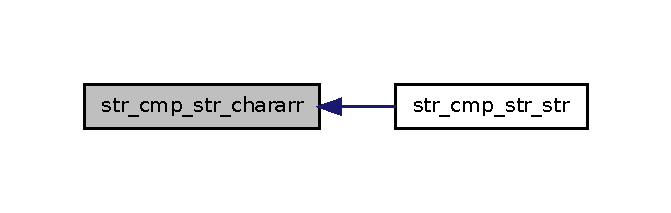
\includegraphics[width=322pt]{str_8c_a0eb24b63eea1db24c63a7d9d1f13aa4d_icgraph}
\end{center}
\end{figure}


\hypertarget{str_8c_a0a559f5efb08d64139c019b1d559fa68}{
\index{str.c@{str.c}!str\_\-cmp\_\-str\_\-str@{str\_\-cmp\_\-str\_\-str}}
\index{str\_\-cmp\_\-str\_\-str@{str\_\-cmp\_\-str\_\-str}!str.c@{str.c}}
\subsubsection[{str\_\-cmp\_\-str\_\-str}]{\setlength{\rightskip}{0pt plus 5cm}int str\_\-cmp\_\-str\_\-str (
\begin{DoxyParamCaption}
\item[{{\bf string}}]{str1, }
\item[{{\bf string}}]{str2}
\end{DoxyParamCaption}
)}}
\label{str_8c_a0a559f5efb08d64139c019b1d559fa68}
Função auxiliar que compara duas estruturas do tipo string.

str1 -\/ estrutura do tipo string  str2 -\/ estrutura do tipo string

inteiro indicando sucesso ou fracasso 

Definição na linha 169 do arquivo str.c.



Este é o diagrama das funções utilizadas por esta função:
\nopagebreak
\begin{figure}[H]
\begin{center}
\leavevmode
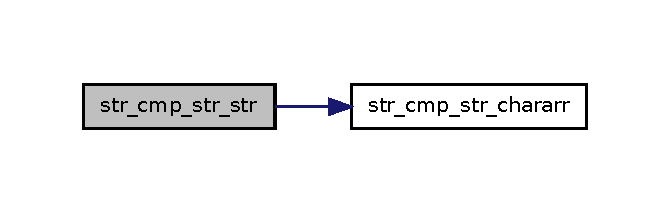
\includegraphics[width=322pt]{str_8c_a0a559f5efb08d64139c019b1d559fa68_cgraph}
\end{center}
\end{figure}


\hypertarget{str_8c_a9c98046afe58b4d941f546c5a604a7de}{
\index{str.c@{str.c}!str\_\-concat\_\-chararr@{str\_\-concat\_\-chararr}}
\index{str\_\-concat\_\-chararr@{str\_\-concat\_\-chararr}!str.c@{str.c}}
\subsubsection[{str\_\-concat\_\-chararr}]{\setlength{\rightskip}{0pt plus 5cm}int str\_\-concat\_\-chararr (
\begin{DoxyParamCaption}
\item[{{\bf string}}]{to, }
\item[{char $\ast$}]{from, }
\item[{size\_\-t}]{num}
\end{DoxyParamCaption}
)}}
\label{str_8c_a9c98046afe58b4d941f546c5a604a7de}
Função auxiliar que concatena uma string 'padrão' com uma estrutura do tipo string

to -\/ estrutura do tipo string  from -\/ string  num -\/ tamanho da string a ser concatenada

inteiro indicando sucesso ou fracasso. 

Definição na linha 106 do arquivo str.c.



Este é o diagrama das funções utilizadas por esta função:
\nopagebreak
\begin{figure}[H]
\begin{center}
\leavevmode
\includegraphics[width=400pt]{str_8c_a9c98046afe58b4d941f546c5a604a7de_cgraph}
\end{center}
\end{figure}




Este é o diagrama das funções que utilizam esta função:
\nopagebreak
\begin{figure}[H]
\begin{center}
\leavevmode
\includegraphics[width=400pt]{str_8c_a9c98046afe58b4d941f546c5a604a7de_icgraph}
\end{center}
\end{figure}


\hypertarget{str_8c_afb165027543e6d9d230117702acdadd0}{
\index{str.c@{str.c}!str\_\-concat\_\-str@{str\_\-concat\_\-str}}
\index{str\_\-concat\_\-str@{str\_\-concat\_\-str}!str.c@{str.c}}
\subsubsection[{str\_\-concat\_\-str}]{\setlength{\rightskip}{0pt plus 5cm}int str\_\-concat\_\-str (
\begin{DoxyParamCaption}
\item[{{\bf string}}]{to, }
\item[{{\bf string}}]{from}
\end{DoxyParamCaption}
)}}
\label{str_8c_afb165027543e6d9d230117702acdadd0}
Função auxiliar que concatena duas estruturas do tipo string.

to -\/ estrutura do tipo string a receber a concatenação  from -\/ estrutura do tipo string a ser concatenada

inteiro indicando sucesso ou fracasso 

Definição na linha 135 do arquivo str.c.



Este é o diagrama das funções utilizadas por esta função:
\nopagebreak
\begin{figure}[H]
\begin{center}
\leavevmode
\includegraphics[width=400pt]{str_8c_afb165027543e6d9d230117702acdadd0_cgraph}
\end{center}
\end{figure}


\hypertarget{str_8c_a0df87a68167272d6191fd0fcef787752}{
\index{str.c@{str.c}!str\_\-cur\_\-size@{str\_\-cur\_\-size}}
\index{str\_\-cur\_\-size@{str\_\-cur\_\-size}!str.c@{str.c}}
\subsubsection[{str\_\-cur\_\-size}]{\setlength{\rightskip}{0pt plus 5cm}size\_\-t str\_\-cur\_\-size (
\begin{DoxyParamCaption}
\item[{{\bf string}}]{str}
\end{DoxyParamCaption}
)}}
\label{str_8c_a0df87a68167272d6191fd0fcef787752}
Função auxiliar que indica o tamanho atual da estrutura do tipod string.

str -\/ estrutura do tipo string

inteiro representando o tamanho atual da string. 

Definição na linha 74 do arquivo str.c.



Este é o diagrama das funções que utilizam esta função:
\nopagebreak
\begin{figure}[H]
\begin{center}
\leavevmode
\includegraphics[width=400pt]{str_8c_a0df87a68167272d6191fd0fcef787752_icgraph}
\end{center}
\end{figure}


\hypertarget{str_8c_a4aa5d752bfb8c556b3566f0b85b07d4d}{
\index{str.c@{str.c}!str\_\-free@{str\_\-free}}
\index{str\_\-free@{str\_\-free}!str.c@{str.c}}
\subsubsection[{str\_\-free}]{\setlength{\rightskip}{0pt plus 5cm}int str\_\-free (
\begin{DoxyParamCaption}
\item[{{\bf string}}]{str}
\end{DoxyParamCaption}
)}}
\label{str_8c_a4aa5d752bfb8c556b3566f0b85b07d4d}
Função auxiliar que libera a memória alocada por uma string

str -\/ estrutura do tipo string

um inteiro descrevendo o sucesso ou falha 

Definição na linha 38 do arquivo str.c.



Este é o diagrama das funções que utilizam esta função:
\nopagebreak
\begin{figure}[H]
\begin{center}
\leavevmode
\includegraphics[width=212pt]{str_8c_a4aa5d752bfb8c556b3566f0b85b07d4d_icgraph}
\end{center}
\end{figure}


\hypertarget{str_8c_a47d6c89b7dacac751de1965e2ee90189}{
\index{str.c@{str.c}!str\_\-free\_\-size@{str\_\-free\_\-size}}
\index{str\_\-free\_\-size@{str\_\-free\_\-size}!str.c@{str.c}}
\subsubsection[{str\_\-free\_\-size}]{\setlength{\rightskip}{0pt plus 5cm}size\_\-t str\_\-free\_\-size (
\begin{DoxyParamCaption}
\item[{{\bf string}}]{str}
\end{DoxyParamCaption}
)}}
\label{str_8c_a47d6c89b7dacac751de1965e2ee90189}
Função auxiliar que mostra quanto há de espaço livre na estrutura de dados do tipo string.

str -\/ estrutura do tipo string

inteiro representando quanto há de espaço livre 

Definição na linha 89 do arquivo str.c.



Este é o diagrama das funções utilizadas por esta função:
\nopagebreak
\begin{figure}[H]
\begin{center}
\leavevmode
\includegraphics[width=274pt]{str_8c_a47d6c89b7dacac751de1965e2ee90189_cgraph}
\end{center}
\end{figure}




Este é o diagrama das funções que utilizam esta função:
\nopagebreak
\begin{figure}[H]
\begin{center}
\leavevmode
\includegraphics[width=400pt]{str_8c_a47d6c89b7dacac751de1965e2ee90189_icgraph}
\end{center}
\end{figure}


\hypertarget{str_8c_a43e9efab3e78f169462b9f842c827fba}{
\index{str.c@{str.c}!str\_\-initialize@{str\_\-initialize}}
\index{str\_\-initialize@{str\_\-initialize}!str.c@{str.c}}
\subsubsection[{str\_\-initialize}]{\setlength{\rightskip}{0pt plus 5cm}{\bf string} str\_\-initialize (
\begin{DoxyParamCaption}
\item[{size\_\-t}]{size}
\end{DoxyParamCaption}
)}}
\label{str_8c_a43e9efab3e78f169462b9f842c827fba}
Função auxiliar que inicializa uma estrututura do tipo string.

size -\/ tamanho da string a ser inicializada

string inicializada 

Definição na linha 14 do arquivo str.c.



Este é o diagrama das funções utilizadas por esta função:
\nopagebreak
\begin{figure}[H]
\begin{center}
\leavevmode
\includegraphics[width=244pt]{str_8c_a43e9efab3e78f169462b9f842c827fba_cgraph}
\end{center}
\end{figure}




Este é o diagrama das funções que utilizam esta função:
\nopagebreak
\begin{figure}[H]
\begin{center}
\leavevmode
\includegraphics[width=400pt]{str_8c_a43e9efab3e78f169462b9f842c827fba_icgraph}
\end{center}
\end{figure}


\hypertarget{str_8c_ae20e94ac638a09b2cd12680cbdae2910}{
\index{str.c@{str.c}!str\_\-max\_\-size@{str\_\-max\_\-size}}
\index{str\_\-max\_\-size@{str\_\-max\_\-size}!str.c@{str.c}}
\subsubsection[{str\_\-max\_\-size}]{\setlength{\rightskip}{0pt plus 5cm}size\_\-t str\_\-max\_\-size (
\begin{DoxyParamCaption}
\item[{{\bf string}}]{str}
\end{DoxyParamCaption}
)}}
\label{str_8c_ae20e94ac638a09b2cd12680cbdae2910}
Função auxiliar que indica o tamanho máximo da estrutura do tipo string.

str -\/ estrutura do tipo string

inteiro descrevendo o tamanho máximo da string. 

Definição na linha 59 do arquivo str.c.



Este é o diagrama das funções que utilizam esta função:
\nopagebreak
\begin{figure}[H]
\begin{center}
\leavevmode
\includegraphics[width=400pt]{str_8c_ae20e94ac638a09b2cd12680cbdae2910_icgraph}
\end{center}
\end{figure}



\hypertarget{str_8h}{
\section{Referência do Arquivo str.h}
\label{str_8h}\index{str.h@{str.h}}
}
{\ttfamily \#include $<$stdio.h$>$}\par
{\ttfamily \#include $<$string.h$>$}\par
{\ttfamily \#include $<$stdlib.h$>$}\par
Gráfico de dependência de inclusões para str.h:
\nopagebreak
\begin{figure}[H]
\begin{center}
\leavevmode
\includegraphics[width=266pt]{str_8h__incl}
\end{center}
\end{figure}
Este grafo mostra quais arquivos estão direta ou indiretamente relacionados com este arquivo:
\nopagebreak
\begin{figure}[H]
\begin{center}
\leavevmode
\includegraphics[width=292pt]{str_8h__dep__incl}
\end{center}
\end{figure}
\subsection*{Estruturas de Dados}
\begin{DoxyCompactItemize}
\item 
struct \hyperlink{structstr}{str}
\end{DoxyCompactItemize}
\subsection*{Definições de Tipos}
\begin{DoxyCompactItemize}
\item 
typedef struct \hyperlink{structstr}{str} $\ast$ \hyperlink{str_8h_a7d94dc8a8cdc32f0385ef28d8c511c52}{string}
\end{DoxyCompactItemize}
\subsection*{Funções}
\begin{DoxyCompactItemize}
\item 
size\_\-t \hyperlink{str_8h_a1dfa00642ae5f5be626f6d5e018fd6ad}{str\_\-max\_\-size} (\hyperlink{structstr}{string} \hyperlink{structstr}{string})
\item 
size\_\-t \hyperlink{str_8h_a8b4c5d297194c9f1f57ca0e79ca31ba4}{str\_\-cur\_\-size} (\hyperlink{structstr}{string} \hyperlink{structstr}{string})
\item 
size\_\-t \hyperlink{str_8h_afa61b1760ef7da2de72524003044f203}{str\_\-free\_\-size} (\hyperlink{structstr}{string} \hyperlink{structstr}{string})
\item 
\hyperlink{structstr}{string} \hyperlink{str_8h_a43e9efab3e78f169462b9f842c827fba}{str\_\-initialize} (size\_\-t size)
\item 
int \hyperlink{str_8h_a5ca723b0fa09efed3e009b907daa44ca}{str\_\-free} (\hyperlink{structstr}{string} \hyperlink{structstr}{string})
\item 
int \hyperlink{str_8h_a0551d9da0243fc76764a50740d442547}{str\_\-concat\_\-chararr} (\hyperlink{structstr}{string} to, char $\ast$from, size\_\-t size)
\item 
int \hyperlink{str_8h_afb165027543e6d9d230117702acdadd0}{str\_\-concat\_\-str} (\hyperlink{structstr}{string} to, \hyperlink{structstr}{string} from)
\item 
int \hyperlink{str_8h_a0eb24b63eea1db24c63a7d9d1f13aa4d}{str\_\-cmp\_\-str\_\-chararr} (\hyperlink{structstr}{string} \hyperlink{structstr}{str}, char $\ast$elt, size\_\-t size)
\item 
int \hyperlink{str_8h_a0a559f5efb08d64139c019b1d559fa68}{str\_\-cmp\_\-str\_\-str} (\hyperlink{structstr}{string} str1, \hyperlink{structstr}{string} str2)
\end{DoxyCompactItemize}


\subsection{Definições dos tipos}
\hypertarget{str_8h_a7d94dc8a8cdc32f0385ef28d8c511c52}{
\index{str.h@{str.h}!string@{string}}
\index{string@{string}!str.h@{str.h}}
\subsubsection[{string}]{\setlength{\rightskip}{0pt plus 5cm}typedef struct {\bf str}$\ast$ {\bf string}}}
\label{str_8h_a7d94dc8a8cdc32f0385ef28d8c511c52}


Definição na linha 24 do arquivo str.h.



\subsection{Funções}
\hypertarget{str_8h_a0eb24b63eea1db24c63a7d9d1f13aa4d}{
\index{str.h@{str.h}!str\_\-cmp\_\-str\_\-chararr@{str\_\-cmp\_\-str\_\-chararr}}
\index{str\_\-cmp\_\-str\_\-chararr@{str\_\-cmp\_\-str\_\-chararr}!str.h@{str.h}}
\subsubsection[{str\_\-cmp\_\-str\_\-chararr}]{\setlength{\rightskip}{0pt plus 5cm}int str\_\-cmp\_\-str\_\-chararr (
\begin{DoxyParamCaption}
\item[{{\bf string}}]{str, }
\item[{char $\ast$}]{elt, }
\item[{size\_\-t}]{size}
\end{DoxyParamCaption}
)}}
\label{str_8h_a0eb24b63eea1db24c63a7d9d1f13aa4d}
Função auxiliar que compara uma estrutura do tipo string com uma string \char`\"{}padrao\char`\"{}.

str -\/ estrutura do tipo string  elt -\/ string  size -\/ tamanho da string

inteiro indicando sucesso ou fracasso 

Definição na linha 152 do arquivo str.c.



Este é o diagrama das funções que utilizam esta função:
\nopagebreak
\begin{figure}[H]
\begin{center}
\leavevmode
\includegraphics[width=322pt]{str_8h_a0eb24b63eea1db24c63a7d9d1f13aa4d_icgraph}
\end{center}
\end{figure}


\hypertarget{str_8h_a0a559f5efb08d64139c019b1d559fa68}{
\index{str.h@{str.h}!str\_\-cmp\_\-str\_\-str@{str\_\-cmp\_\-str\_\-str}}
\index{str\_\-cmp\_\-str\_\-str@{str\_\-cmp\_\-str\_\-str}!str.h@{str.h}}
\subsubsection[{str\_\-cmp\_\-str\_\-str}]{\setlength{\rightskip}{0pt plus 5cm}int str\_\-cmp\_\-str\_\-str (
\begin{DoxyParamCaption}
\item[{{\bf string}}]{str1, }
\item[{{\bf string}}]{str2}
\end{DoxyParamCaption}
)}}
\label{str_8h_a0a559f5efb08d64139c019b1d559fa68}
Função auxiliar que compara duas estruturas do tipo string.

str1 -\/ estrutura do tipo string  str2 -\/ estrutura do tipo string

inteiro indicando sucesso ou fracasso 

Definição na linha 169 do arquivo str.c.



Este é o diagrama das funções utilizadas por esta função:
\nopagebreak
\begin{figure}[H]
\begin{center}
\leavevmode
\includegraphics[width=322pt]{str_8h_a0a559f5efb08d64139c019b1d559fa68_cgraph}
\end{center}
\end{figure}


\hypertarget{str_8h_a0551d9da0243fc76764a50740d442547}{
\index{str.h@{str.h}!str\_\-concat\_\-chararr@{str\_\-concat\_\-chararr}}
\index{str\_\-concat\_\-chararr@{str\_\-concat\_\-chararr}!str.h@{str.h}}
\subsubsection[{str\_\-concat\_\-chararr}]{\setlength{\rightskip}{0pt plus 5cm}int str\_\-concat\_\-chararr (
\begin{DoxyParamCaption}
\item[{{\bf string}}]{to, }
\item[{char $\ast$}]{from, }
\item[{size\_\-t}]{num}
\end{DoxyParamCaption}
)}}
\label{str_8h_a0551d9da0243fc76764a50740d442547}
Função auxiliar que concatena uma string 'padrão' com uma estrutura do tipo string

to -\/ estrutura do tipo string  from -\/ string  num -\/ tamanho da string a ser concatenada

inteiro indicando sucesso ou fracasso. 

Definição na linha 106 do arquivo str.c.



Este é o diagrama das funções utilizadas por esta função:
\nopagebreak
\begin{figure}[H]
\begin{center}
\leavevmode
\includegraphics[width=400pt]{str_8h_a0551d9da0243fc76764a50740d442547_cgraph}
\end{center}
\end{figure}




Este é o diagrama das funções que utilizam esta função:
\nopagebreak
\begin{figure}[H]
\begin{center}
\leavevmode
\includegraphics[width=400pt]{str_8h_a0551d9da0243fc76764a50740d442547_icgraph}
\end{center}
\end{figure}


\hypertarget{str_8h_afb165027543e6d9d230117702acdadd0}{
\index{str.h@{str.h}!str\_\-concat\_\-str@{str\_\-concat\_\-str}}
\index{str\_\-concat\_\-str@{str\_\-concat\_\-str}!str.h@{str.h}}
\subsubsection[{str\_\-concat\_\-str}]{\setlength{\rightskip}{0pt plus 5cm}int str\_\-concat\_\-str (
\begin{DoxyParamCaption}
\item[{{\bf string}}]{to, }
\item[{{\bf string}}]{from}
\end{DoxyParamCaption}
)}}
\label{str_8h_afb165027543e6d9d230117702acdadd0}
Função auxiliar que concatena duas estruturas do tipo string.

to -\/ estrutura do tipo string a receber a concatenação  from -\/ estrutura do tipo string a ser concatenada

inteiro indicando sucesso ou fracasso 

Definição na linha 135 do arquivo str.c.



Este é o diagrama das funções utilizadas por esta função:
\nopagebreak
\begin{figure}[H]
\begin{center}
\leavevmode
\includegraphics[width=400pt]{str_8h_afb165027543e6d9d230117702acdadd0_cgraph}
\end{center}
\end{figure}


\hypertarget{str_8h_a8b4c5d297194c9f1f57ca0e79ca31ba4}{
\index{str.h@{str.h}!str\_\-cur\_\-size@{str\_\-cur\_\-size}}
\index{str\_\-cur\_\-size@{str\_\-cur\_\-size}!str.h@{str.h}}
\subsubsection[{str\_\-cur\_\-size}]{\setlength{\rightskip}{0pt plus 5cm}size\_\-t str\_\-cur\_\-size (
\begin{DoxyParamCaption}
\item[{{\bf string}}]{str}
\end{DoxyParamCaption}
)}}
\label{str_8h_a8b4c5d297194c9f1f57ca0e79ca31ba4}
Função auxiliar que indica o tamanho atual da estrutura do tipod string.

str -\/ estrutura do tipo string

inteiro representando o tamanho atual da string. 

Definição na linha 74 do arquivo str.c.



Este é o diagrama das funções que utilizam esta função:
\nopagebreak
\begin{figure}[H]
\begin{center}
\leavevmode
\includegraphics[width=400pt]{str_8h_a8b4c5d297194c9f1f57ca0e79ca31ba4_icgraph}
\end{center}
\end{figure}


\hypertarget{str_8h_a5ca723b0fa09efed3e009b907daa44ca}{
\index{str.h@{str.h}!str\_\-free@{str\_\-free}}
\index{str\_\-free@{str\_\-free}!str.h@{str.h}}
\subsubsection[{str\_\-free}]{\setlength{\rightskip}{0pt plus 5cm}int str\_\-free (
\begin{DoxyParamCaption}
\item[{{\bf string}}]{str}
\end{DoxyParamCaption}
)}}
\label{str_8h_a5ca723b0fa09efed3e009b907daa44ca}
Função auxiliar que libera a memória alocada por uma string

str -\/ estrutura do tipo string

um inteiro descrevendo o sucesso ou falha 

Definição na linha 38 do arquivo str.c.



Este é o diagrama das funções que utilizam esta função:
\nopagebreak
\begin{figure}[H]
\begin{center}
\leavevmode
\includegraphics[width=212pt]{str_8h_a5ca723b0fa09efed3e009b907daa44ca_icgraph}
\end{center}
\end{figure}


\hypertarget{str_8h_afa61b1760ef7da2de72524003044f203}{
\index{str.h@{str.h}!str\_\-free\_\-size@{str\_\-free\_\-size}}
\index{str\_\-free\_\-size@{str\_\-free\_\-size}!str.h@{str.h}}
\subsubsection[{str\_\-free\_\-size}]{\setlength{\rightskip}{0pt plus 5cm}size\_\-t str\_\-free\_\-size (
\begin{DoxyParamCaption}
\item[{{\bf string}}]{str}
\end{DoxyParamCaption}
)}}
\label{str_8h_afa61b1760ef7da2de72524003044f203}
Função auxiliar que mostra quanto há de espaço livre na estrutura de dados do tipo string.

str -\/ estrutura do tipo string

inteiro representando quanto há de espaço livre 

Definição na linha 89 do arquivo str.c.



Este é o diagrama das funções utilizadas por esta função:
\nopagebreak
\begin{figure}[H]
\begin{center}
\leavevmode
\includegraphics[width=274pt]{str_8h_afa61b1760ef7da2de72524003044f203_cgraph}
\end{center}
\end{figure}




Este é o diagrama das funções que utilizam esta função:
\nopagebreak
\begin{figure}[H]
\begin{center}
\leavevmode
\includegraphics[width=400pt]{str_8h_afa61b1760ef7da2de72524003044f203_icgraph}
\end{center}
\end{figure}


\hypertarget{str_8h_a43e9efab3e78f169462b9f842c827fba}{
\index{str.h@{str.h}!str\_\-initialize@{str\_\-initialize}}
\index{str\_\-initialize@{str\_\-initialize}!str.h@{str.h}}
\subsubsection[{str\_\-initialize}]{\setlength{\rightskip}{0pt plus 5cm}{\bf string} str\_\-initialize (
\begin{DoxyParamCaption}
\item[{size\_\-t}]{size}
\end{DoxyParamCaption}
)}}
\label{str_8h_a43e9efab3e78f169462b9f842c827fba}
Função auxiliar que inicializa uma estrututura do tipo string.

size -\/ tamanho da string a ser inicializada

string inicializada 

Definição na linha 14 do arquivo str.c.



Este é o diagrama das funções utilizadas por esta função:
\nopagebreak
\begin{figure}[H]
\begin{center}
\leavevmode
\includegraphics[width=244pt]{str_8h_a43e9efab3e78f169462b9f842c827fba_cgraph}
\end{center}
\end{figure}




Este é o diagrama das funções que utilizam esta função:
\nopagebreak
\begin{figure}[H]
\begin{center}
\leavevmode
\includegraphics[width=400pt]{str_8h_a43e9efab3e78f169462b9f842c827fba_icgraph}
\end{center}
\end{figure}


\hypertarget{str_8h_a1dfa00642ae5f5be626f6d5e018fd6ad}{
\index{str.h@{str.h}!str\_\-max\_\-size@{str\_\-max\_\-size}}
\index{str\_\-max\_\-size@{str\_\-max\_\-size}!str.h@{str.h}}
\subsubsection[{str\_\-max\_\-size}]{\setlength{\rightskip}{0pt plus 5cm}size\_\-t str\_\-max\_\-size (
\begin{DoxyParamCaption}
\item[{{\bf string}}]{str}
\end{DoxyParamCaption}
)}}
\label{str_8h_a1dfa00642ae5f5be626f6d5e018fd6ad}
Função auxiliar que indica o tamanho máximo da estrutura do tipo string.

str -\/ estrutura do tipo string

inteiro descrevendo o tamanho máximo da string. 

Definição na linha 59 do arquivo str.c.



Este é o diagrama das funções que utilizam esta função:
\nopagebreak
\begin{figure}[H]
\begin{center}
\leavevmode
\includegraphics[width=400pt]{str_8h_a1dfa00642ae5f5be626f6d5e018fd6ad_icgraph}
\end{center}
\end{figure}



\hypertarget{tempo_8c}{
\section{Referência do Arquivo tempo.c}
\label{tempo_8c}\index{tempo.c@{tempo.c}}
}
{\ttfamily \#include \char`\"{}tempo.h\char`\"{}}\par
Gráfico de dependência de inclusões para tempo.c:
\nopagebreak
\begin{figure}[H]
\begin{center}
\leavevmode
\includegraphics[width=146pt]{tempo_8c__incl}
\end{center}
\end{figure}
\subsection*{Funções}
\begin{DoxyCompactItemize}
\item 
double \hyperlink{tempo_8c_afa8cb739ea2c6f04b660789e2e36e9ee}{calculaTempo} (struct timeval startTime, struct timeval endTime)
\end{DoxyCompactItemize}


\subsection{Funções}
\hypertarget{tempo_8c_afa8cb739ea2c6f04b660789e2e36e9ee}{
\index{tempo.c@{tempo.c}!calculaTempo@{calculaTempo}}
\index{calculaTempo@{calculaTempo}!tempo.c@{tempo.c}}
\subsubsection[{calculaTempo}]{\setlength{\rightskip}{0pt plus 5cm}double calculaTempo (
\begin{DoxyParamCaption}
\item[{struct timeval}]{startTime, }
\item[{struct timeval}]{endTime}
\end{DoxyParamCaption}
)}}
\label{tempo_8c_afa8cb739ea2c6f04b660789e2e36e9ee}
Função que realiza o cálculo do tempo percorrido em microsegundos, dado um tempo de início e um tempo de fim.

startTime -\/ tempo de início da contagem  endTime -\/ tempo de fim da contagem

tempo percorrido em microsegundos 

Definição na linha 23 do arquivo tempo.c.



Este é o diagrama das funções que utilizam esta função:
\nopagebreak
\begin{figure}[H]
\begin{center}
\leavevmode
\includegraphics[width=240pt]{tempo_8c_afa8cb739ea2c6f04b660789e2e36e9ee_icgraph}
\end{center}
\end{figure}



\hypertarget{tempo_8h}{
\section{Referência do Arquivo tempo.h}
\label{tempo_8h}\index{tempo.h@{tempo.h}}
}
{\ttfamily \#include $<$sys/time.h$>$}\par
Gráfico de dependência de inclusões para tempo.h:
\nopagebreak
\begin{figure}[H]
\begin{center}
\leavevmode
\includegraphics[width=146pt]{tempo_8h__incl}
\end{center}
\end{figure}
Este grafo mostra quais arquivos estão direta ou indiretamente relacionados com este arquivo:
\nopagebreak
\begin{figure}[H]
\begin{center}
\leavevmode
\includegraphics[width=320pt]{tempo_8h__dep__incl}
\end{center}
\end{figure}
\subsection*{Funções}
\begin{DoxyCompactItemize}
\item 
double \hyperlink{tempo_8h_afa8cb739ea2c6f04b660789e2e36e9ee}{calculaTempo} (struct timeval startTime, struct timeval endTime)
\end{DoxyCompactItemize}


\subsection{Funções}
\hypertarget{tempo_8h_afa8cb739ea2c6f04b660789e2e36e9ee}{
\index{tempo.h@{tempo.h}!calculaTempo@{calculaTempo}}
\index{calculaTempo@{calculaTempo}!tempo.h@{tempo.h}}
\subsubsection[{calculaTempo}]{\setlength{\rightskip}{0pt plus 5cm}double calculaTempo (
\begin{DoxyParamCaption}
\item[{struct timeval}]{startTime, }
\item[{struct timeval}]{endTime}
\end{DoxyParamCaption}
)}}
\label{tempo_8h_afa8cb739ea2c6f04b660789e2e36e9ee}
Função que realiza o cálculo do tempo percorrido em microsegundos, dado um tempo de início e um tempo de fim.

startTime -\/ tempo de início da contagem  endTime -\/ tempo de fim da contagem

tempo percorrido em microsegundos 

Definição na linha 23 do arquivo tempo.c.



Este é o diagrama das funções que utilizam esta função:
\nopagebreak
\begin{figure}[H]
\begin{center}
\leavevmode
\includegraphics[width=240pt]{tempo_8h_afa8cb739ea2c6f04b660789e2e36e9ee_icgraph}
\end{center}
\end{figure}



\printindex
\end{document}
